\section[Spectral ViT]{Creation and Training of the Spectral ViT}
%%%%%%%%%%%%%%%%%%%%%%%%%%%%%%%%%%%%%%%%%%%%%%%%%%%%%%%%%%%%%%%%%%%%%%%%
%%%%%%%%%%%%%%%%%%%%%%%%%%%%%%%%%%%%%%%%%%%%%%%%%%%%%%%%%%%%%%%%%%%%%%%%
\begin{frame}{Spectral ViT}
\begin{columns}[c]
\column{.4\textwidth}
Transformer architecture must satisfy 
    \begin{itemize}
        \item 1D Nature of Spectra (more like original transformer)
        \item Cut up data into `patches' synthetically (more like ViT)
    \end{itemize}
\column{.5\textwidth}
    \begin{figure}
        \centering
        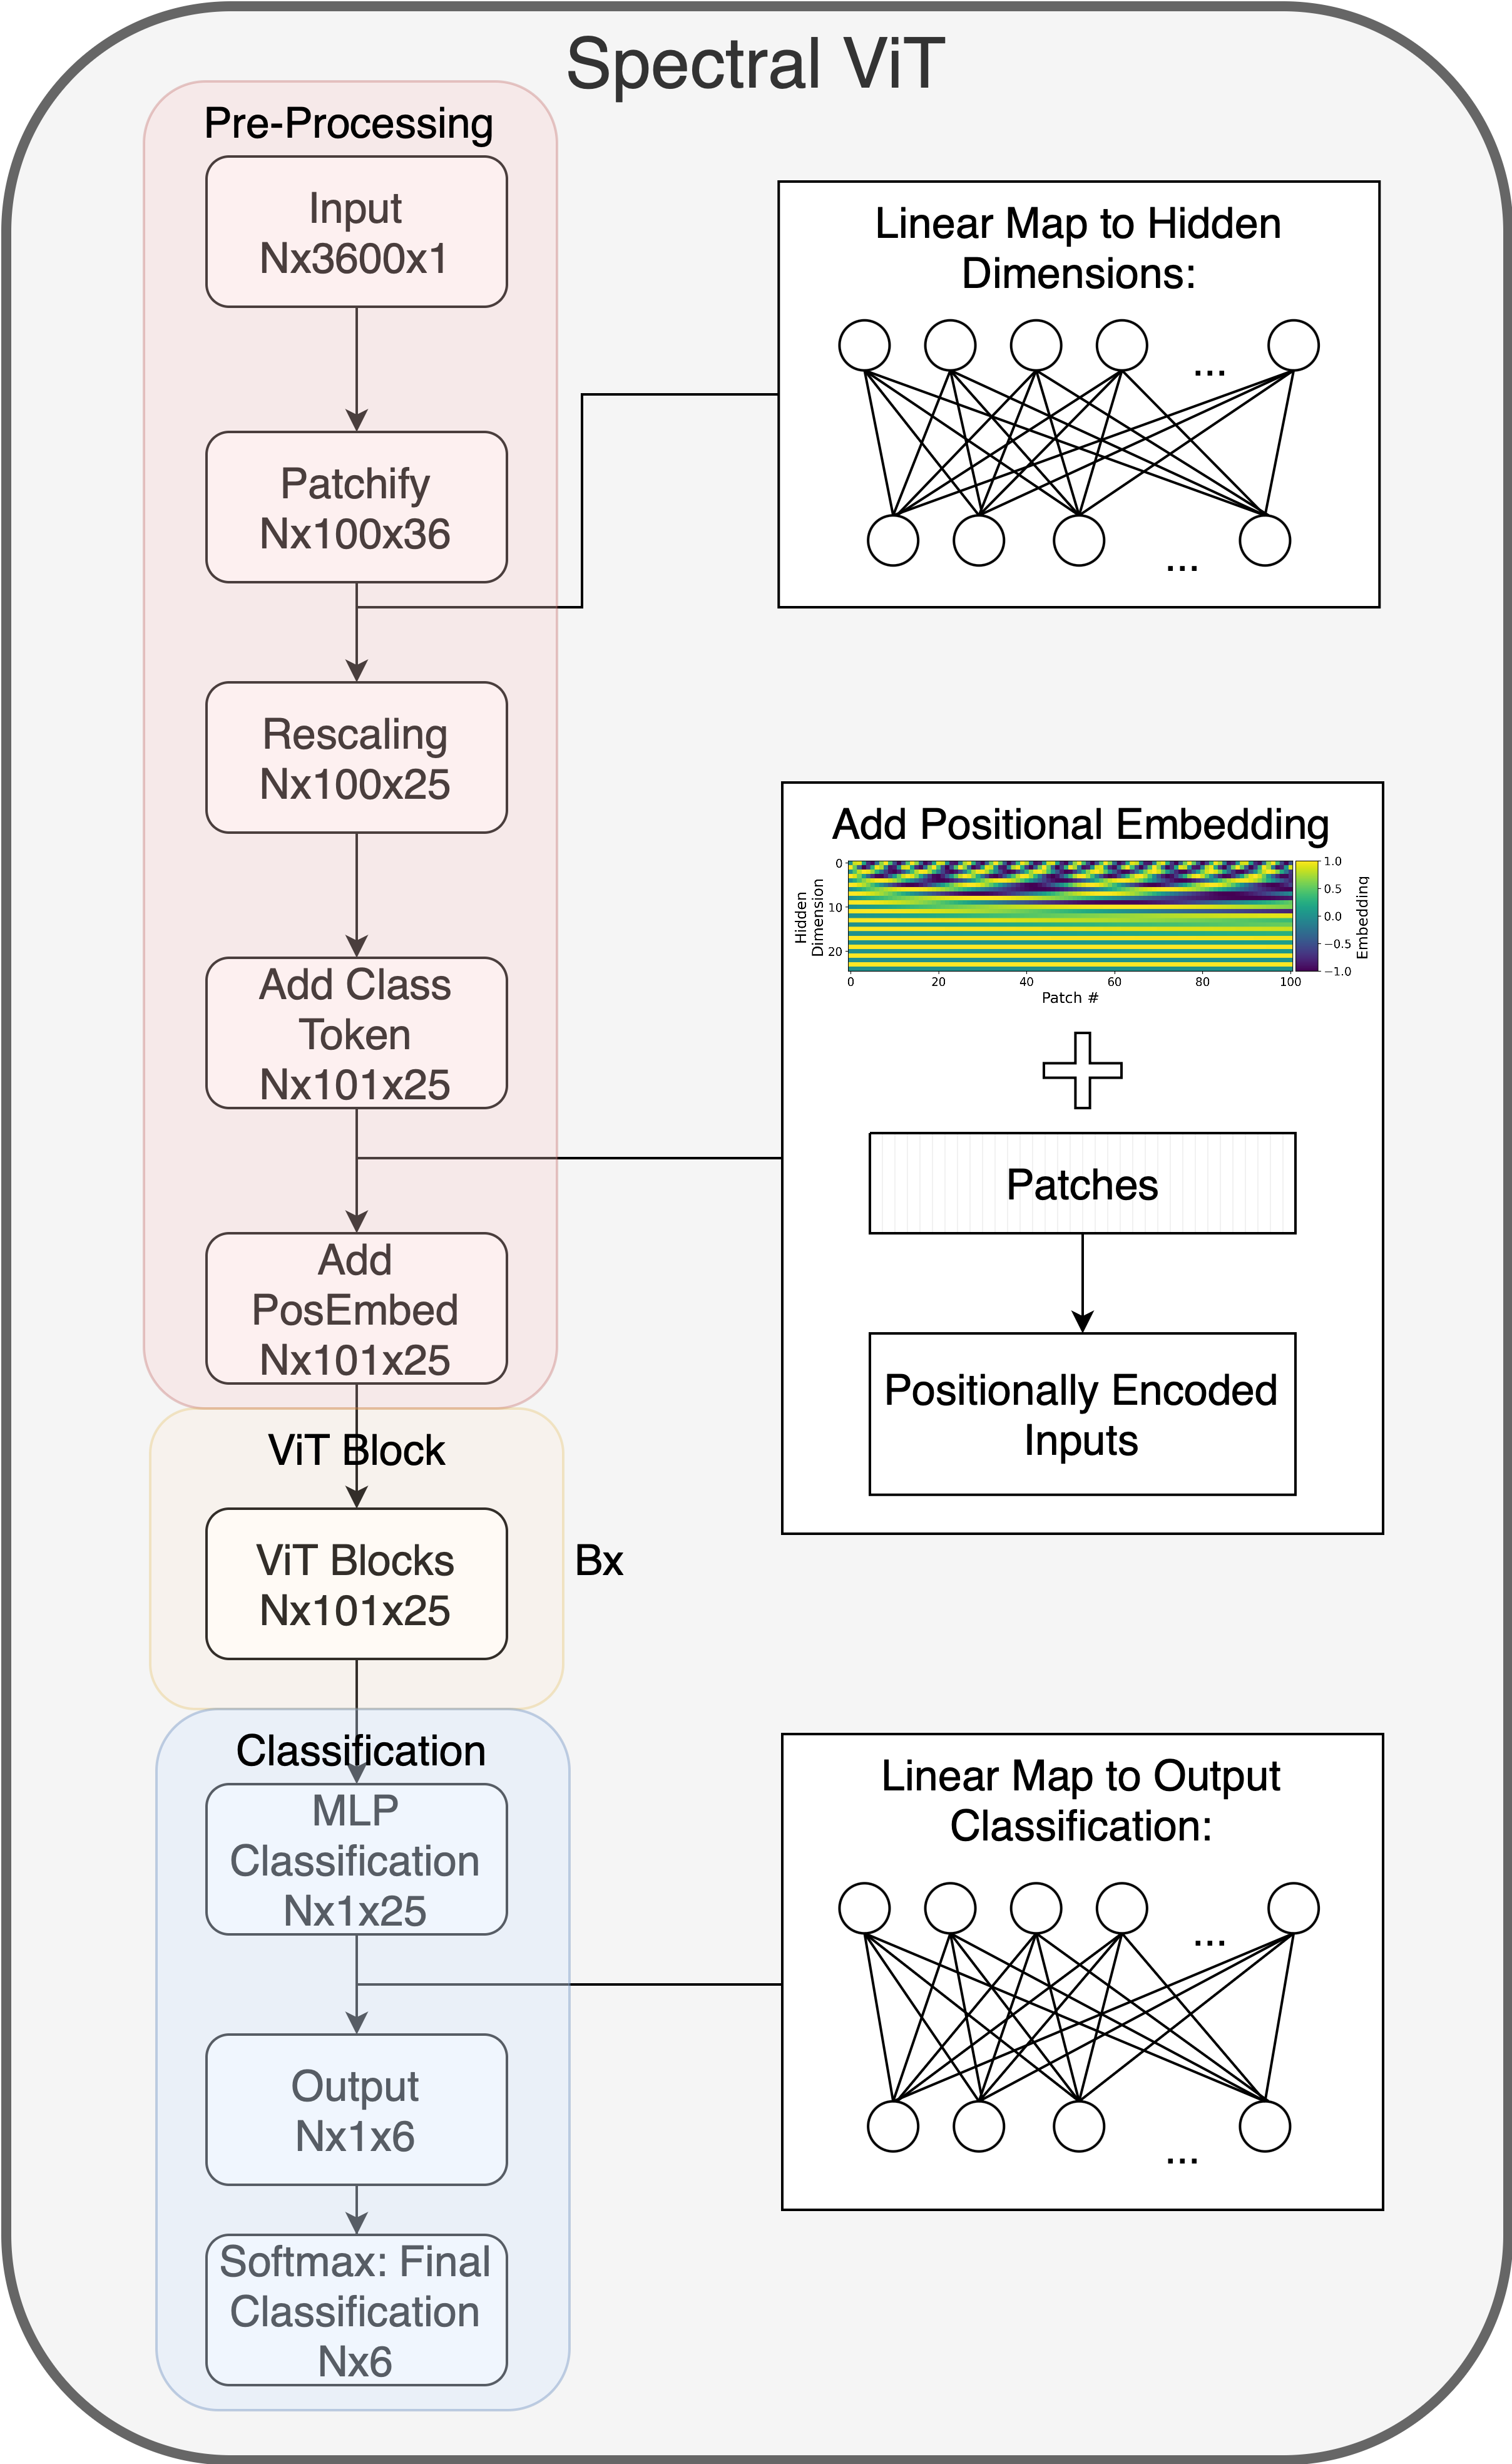
\includegraphics[width=.8\textwidth]{figures/TransformerDiagrams/SpectralViT_Presentation.png}
    \end{figure}
\end{columns}
\end{frame}

%%%%%%%%%%%%%%%%%%%%%%%%%%%%%%%%%%%%%%%%%%%%%%%%%%%%%%%%%%%%%%%%%%%%%%%%
\begin{frame}{Positional Embedding}
    \begin{equation}
        \text{Embedding}_{ij} = \begin{cases} \sin\left(\frac{i}{10000^{(j / \text{patch size})}}\right) & \text{if } j \text{ is even} \\
        \cos\left(\frac{i}{10000^{((j - 1) / \text{patch size})}}\right) & \text{if } j \text{ is odd}\end{cases}
    \end{equation}
    \pause
    \begin{figure}[t]
        \centering
        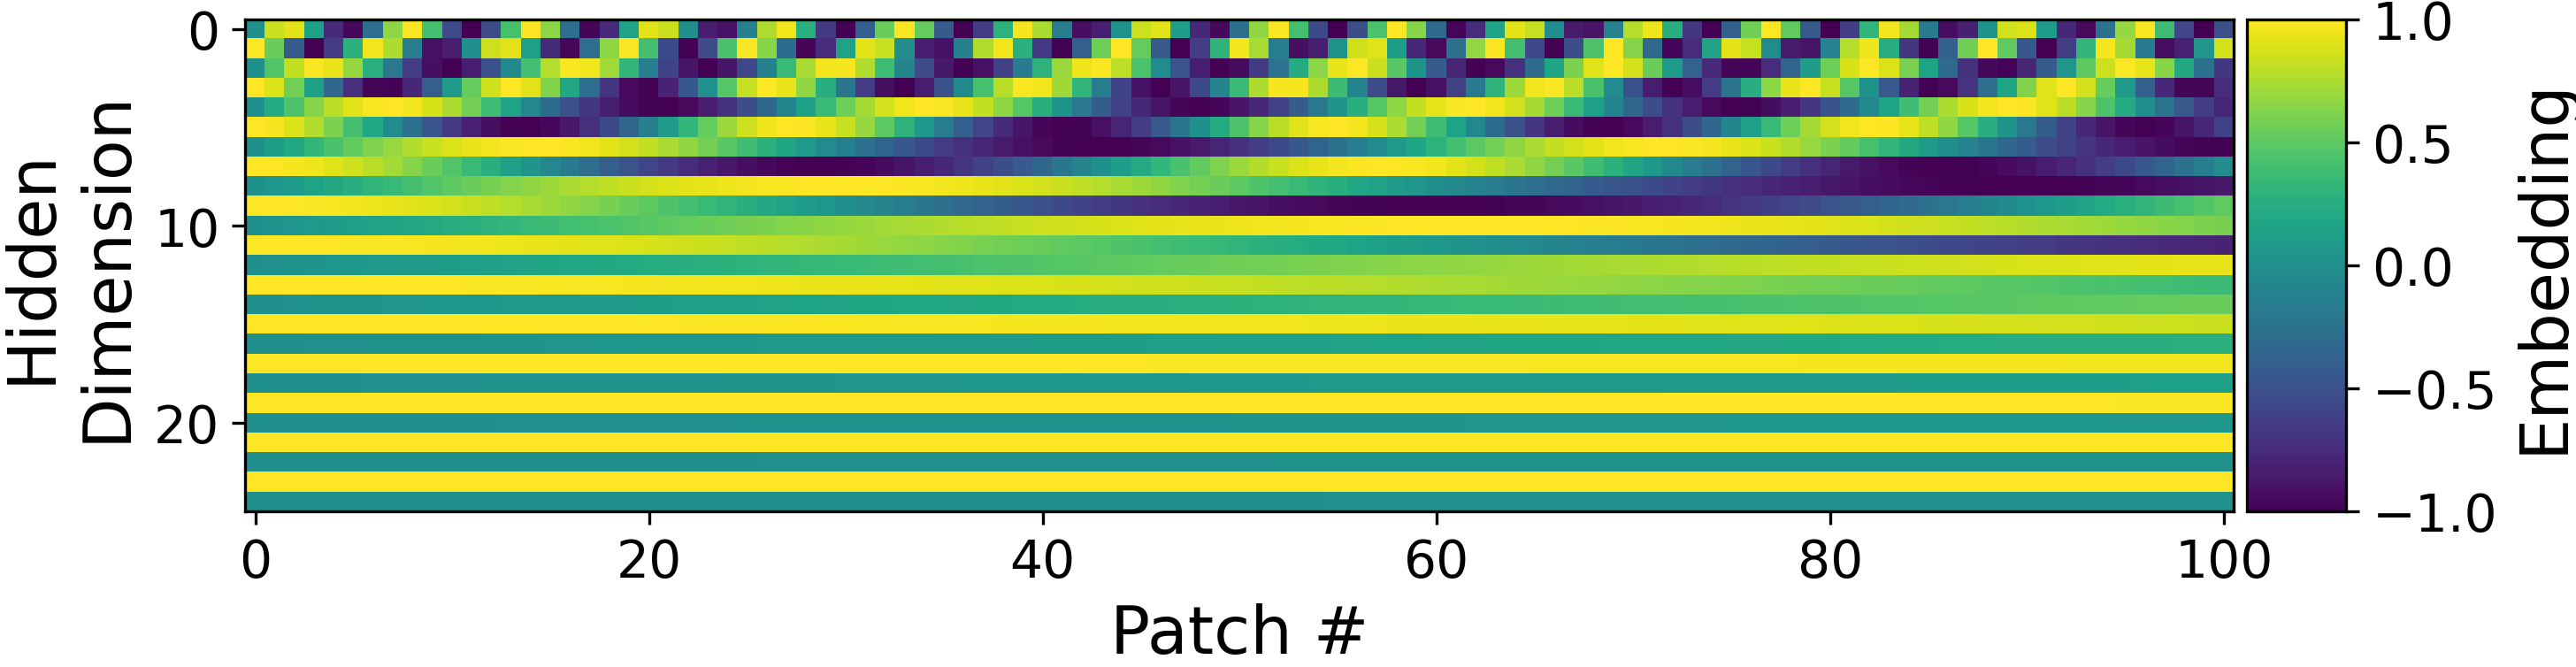
\includegraphics[width=.9\linewidth]{figures/embeddings_new.png}
        \caption{Positional Embeddings for ViT}
    %     {Visual representation of the embeddings for a sample of spectra. The x-axis represents the 
    %     index of the patch, the y-axis represents the index of the hidden dimension, and the color represents 
    % the value of the embedding.}
        \label{fig:embedding}
    \end{figure}
\end{frame}

%%%%%%%%%%%%%%%%%%%%%%%%%%%%%%%%%%%%%%%%%%%%%%%%%%%%%%%%%%%%%%%%%%%%%%%%
\begin{frame}{Attention}
    \begin{equation}
        \label{eq:mhsa}
        \text{Attention}(Q, K, V) = \text{softmax}\left(\frac{Q\cdot K^T}{\sqrt{d_k}}\right)\cdot V
    \end{equation}
    \pause
    \begin{figure}
        \centering 
        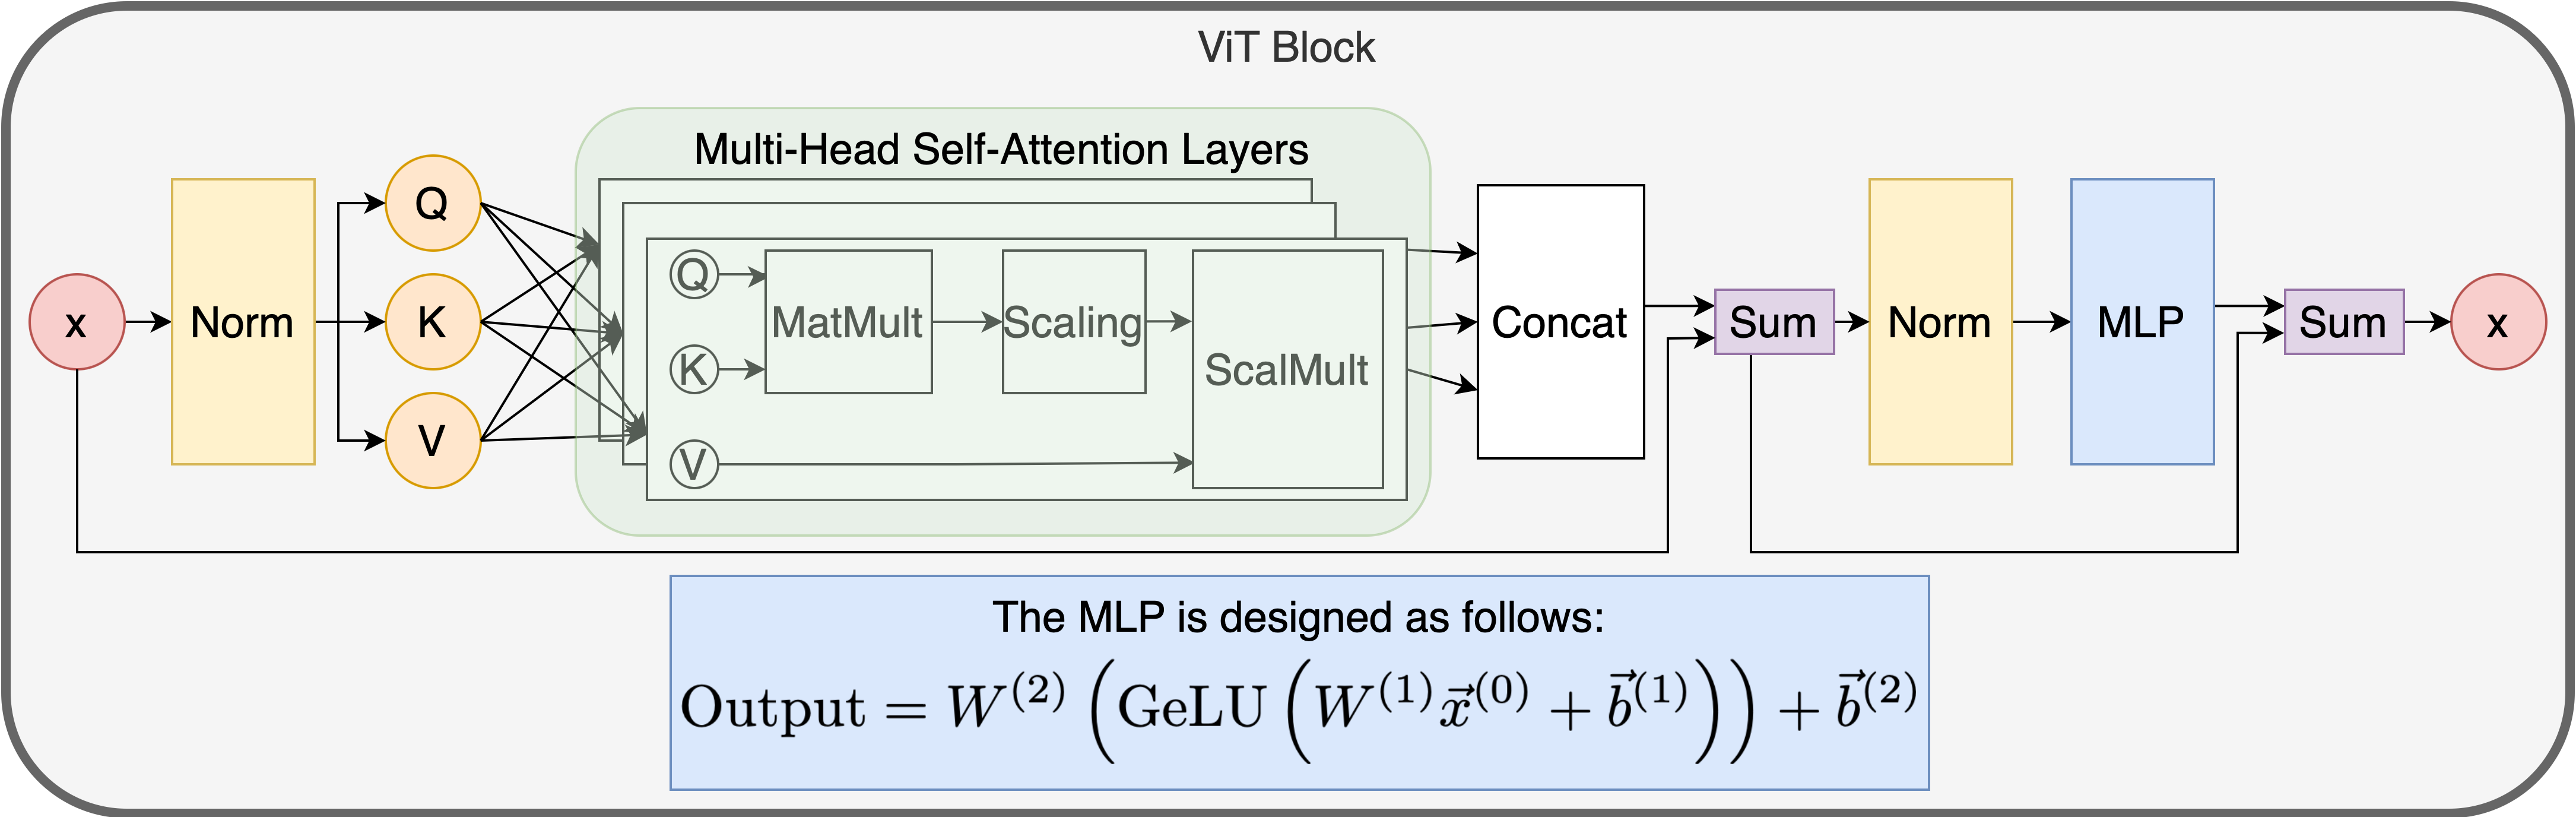
\includegraphics[width=.9\textwidth]{figures/TransformerDiagrams/Attention_Presentation.png}
        \caption{ViT Block Architecture for the Spectral ViT}
        \label{fig:SpectralViTBlock}
    \end{figure}
\end{frame}

%%%%%%%%%%%%%%%%%%%%%%%%%%%%%%%%%%%%%%%%%%%%%%%%%%%%%%%%%%%%%%%%%%%%%%%%
\begin{frame}{Final Architecture}
\begin{columns}[c]
\column{.38\textwidth}
    \begin{figure}
        \centering
        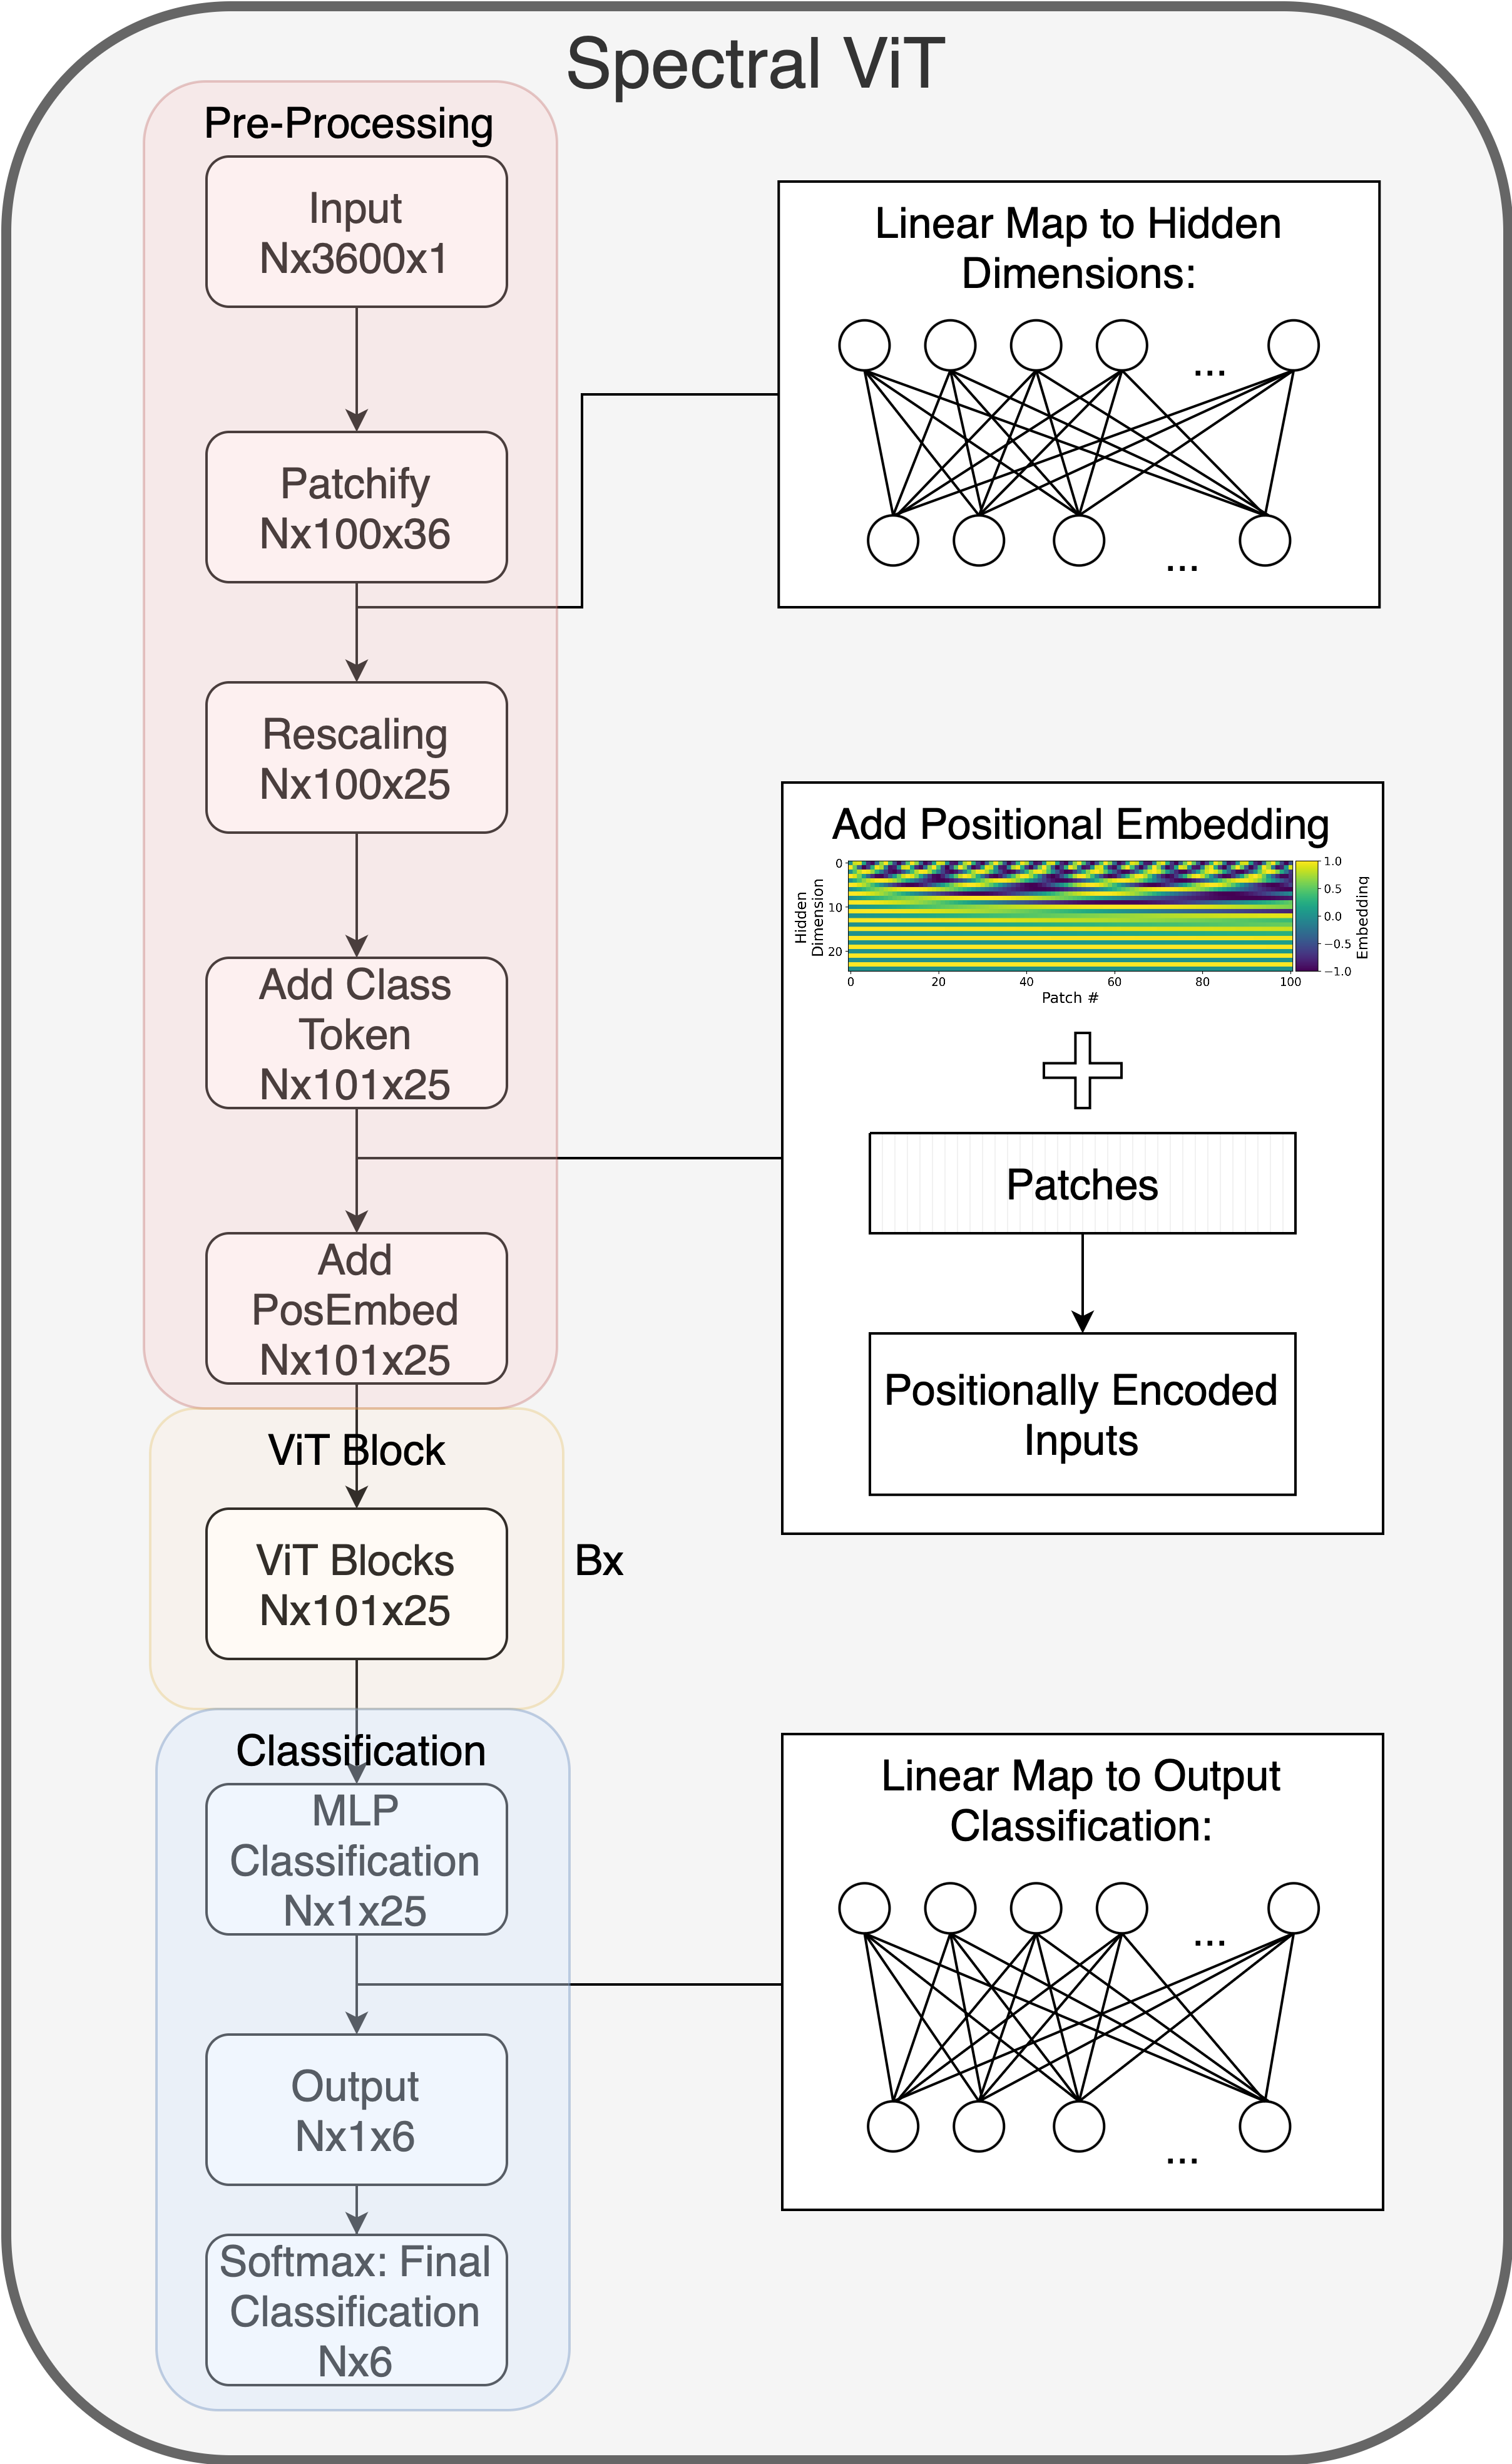
\includegraphics[width=\textwidth]{figures/TransformerDiagrams/SpectralViT_Presentation.png}
    \end{figure}
\column{.58\textwidth}
    \begin{figure}
        \centering
        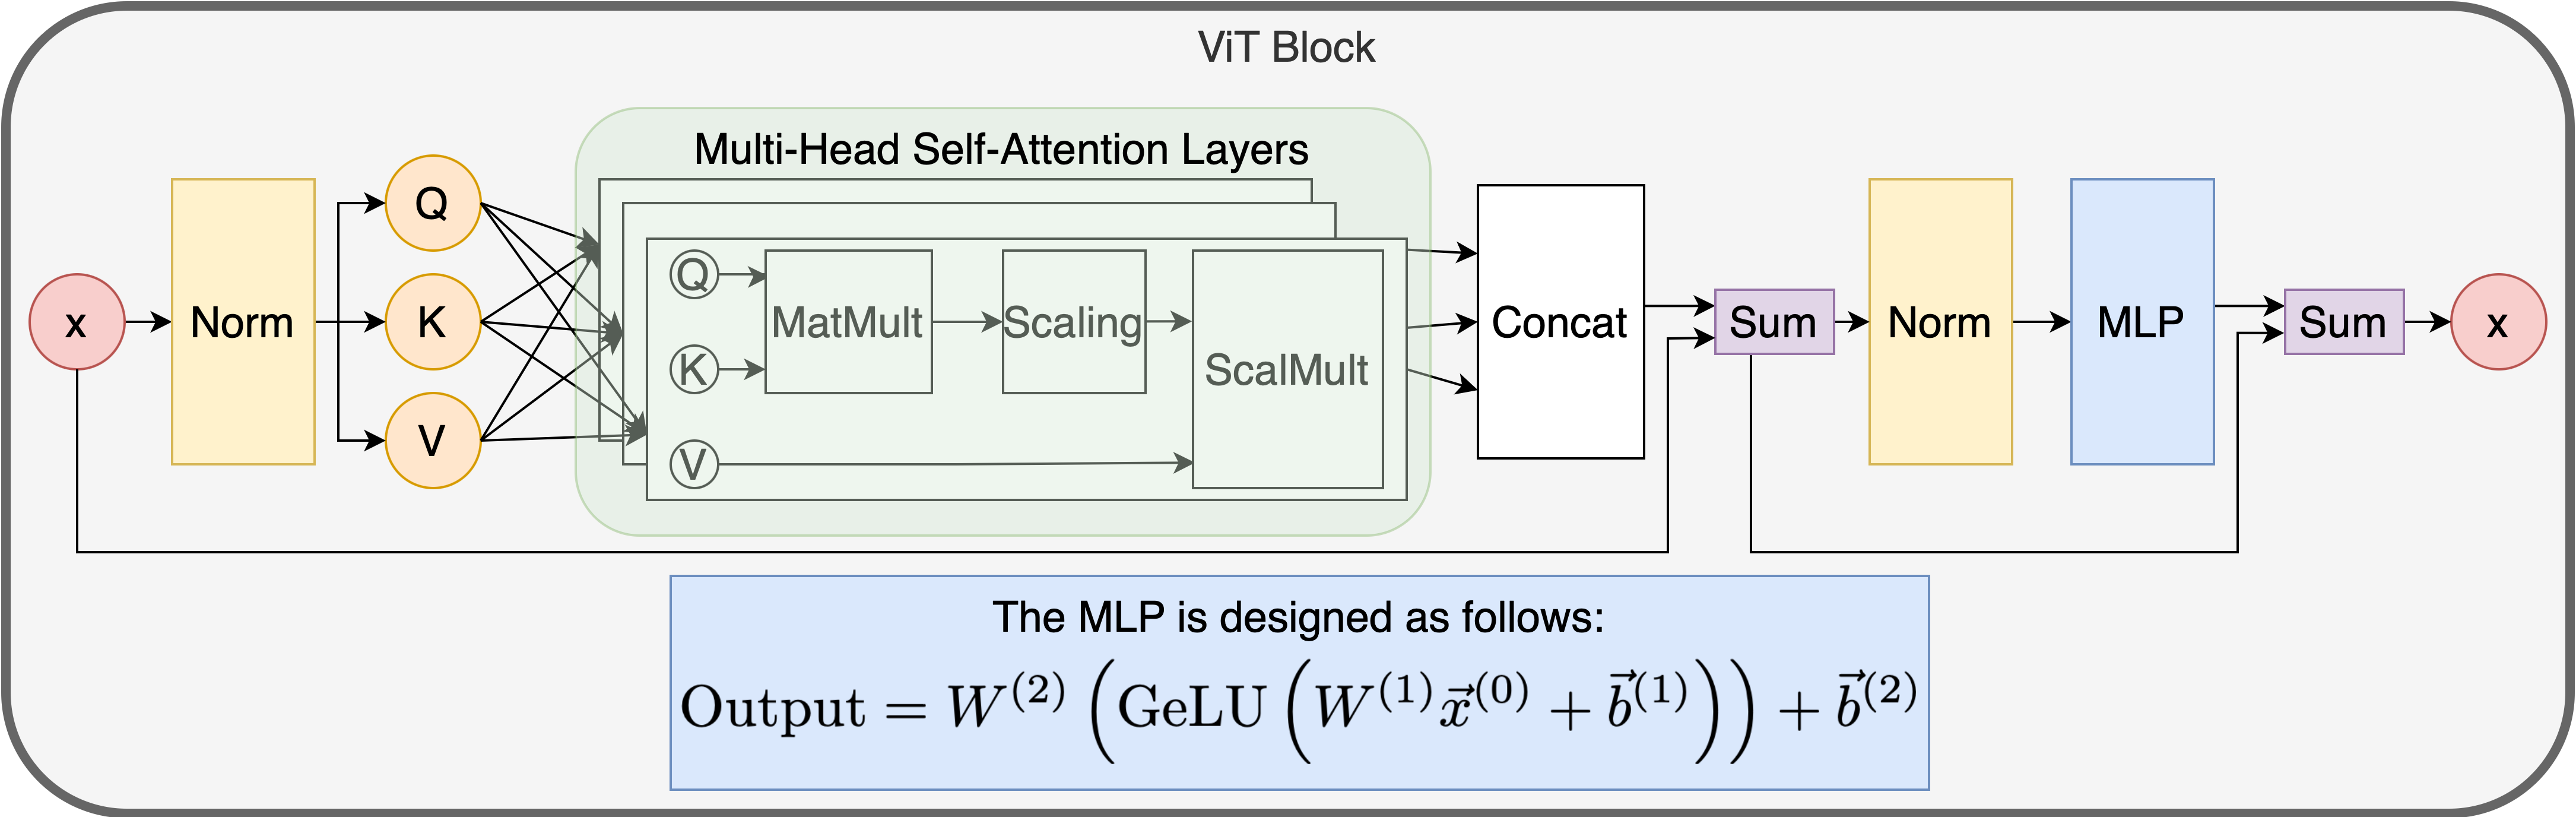
\includegraphics[width=\textwidth]{figures/TransformerDiagrams/Attention_Presentation.png}
    \end{figure}
\end{columns}
\end{frame}
%%%%%%%%%%%%%%%%%%%%%%%%%%%%%%%%%%%%%%%%%%%%%%%%%%%%%%%%%%%%%%%%%%%%%%%%
\begin{frame}
    \begin{figure}[t]
        \centering
        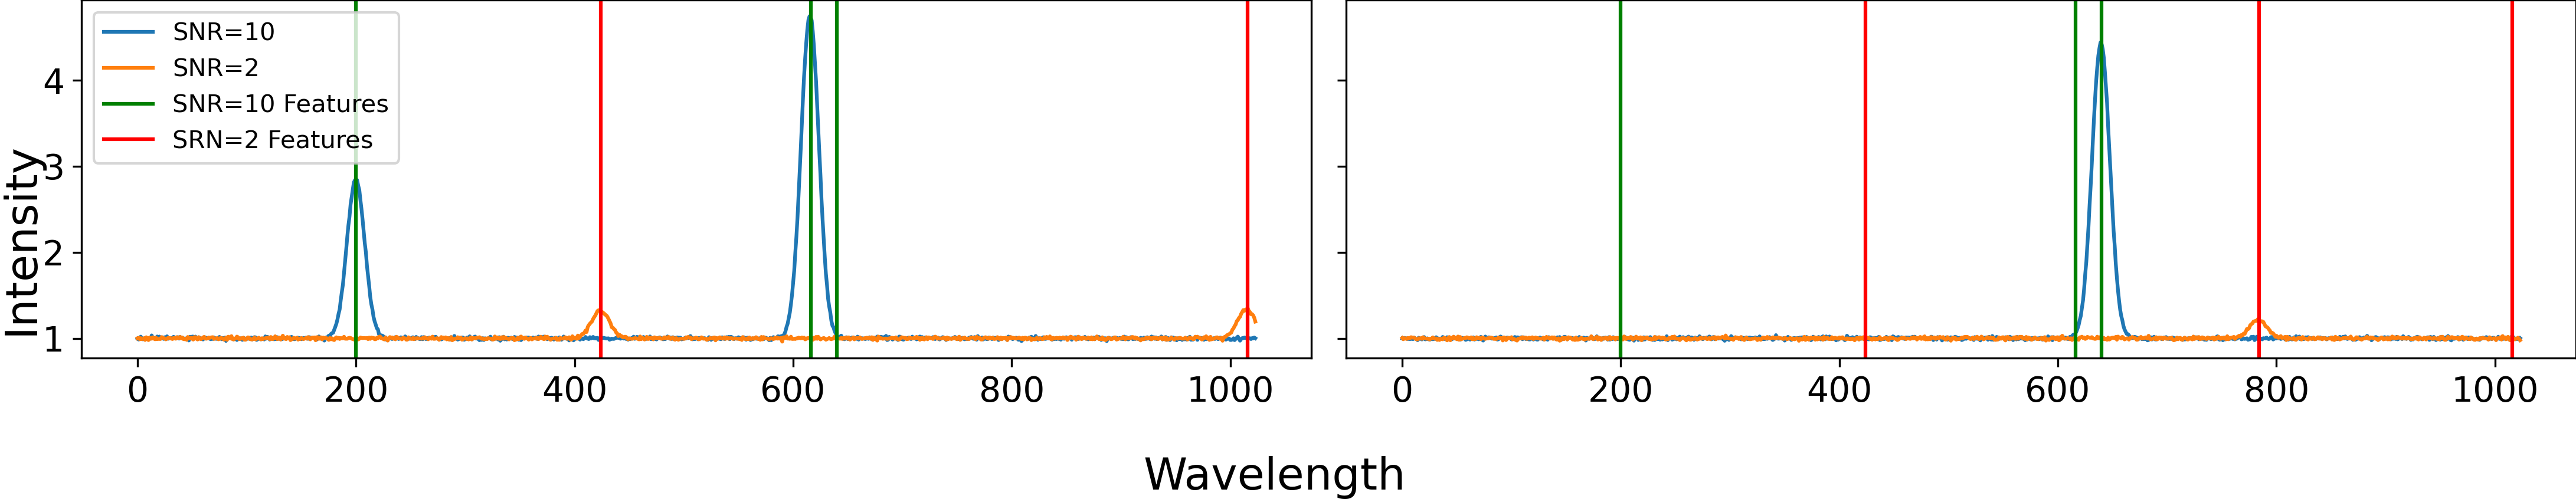
\includegraphics[width=\textwidth]{figures/synth_data_new.png}
        \caption[Synthetic spectra]{Synthetic spectra used to verify the performance of Spectral~ViT. Red and green vertical lines represent features used to 
        separate the data into distinct classes for SNR=2 and SNR=10, respectively. Two classes are shown for each SNR.}
        \label{fig:synth_spectra}
    \end{figure}
\end{frame}


%%%%%%%%%%%%%%%%%%%%%%%%%%%%%%%%%%%%%%%%%%%%%%%%%%%%%%%%%%%%%%%%%%%%%%%%
\begin{frame}
    \begin{figure}[t]
        \centering
        \subfloat[\centering~SNR = 2\label{fig:snr2}]{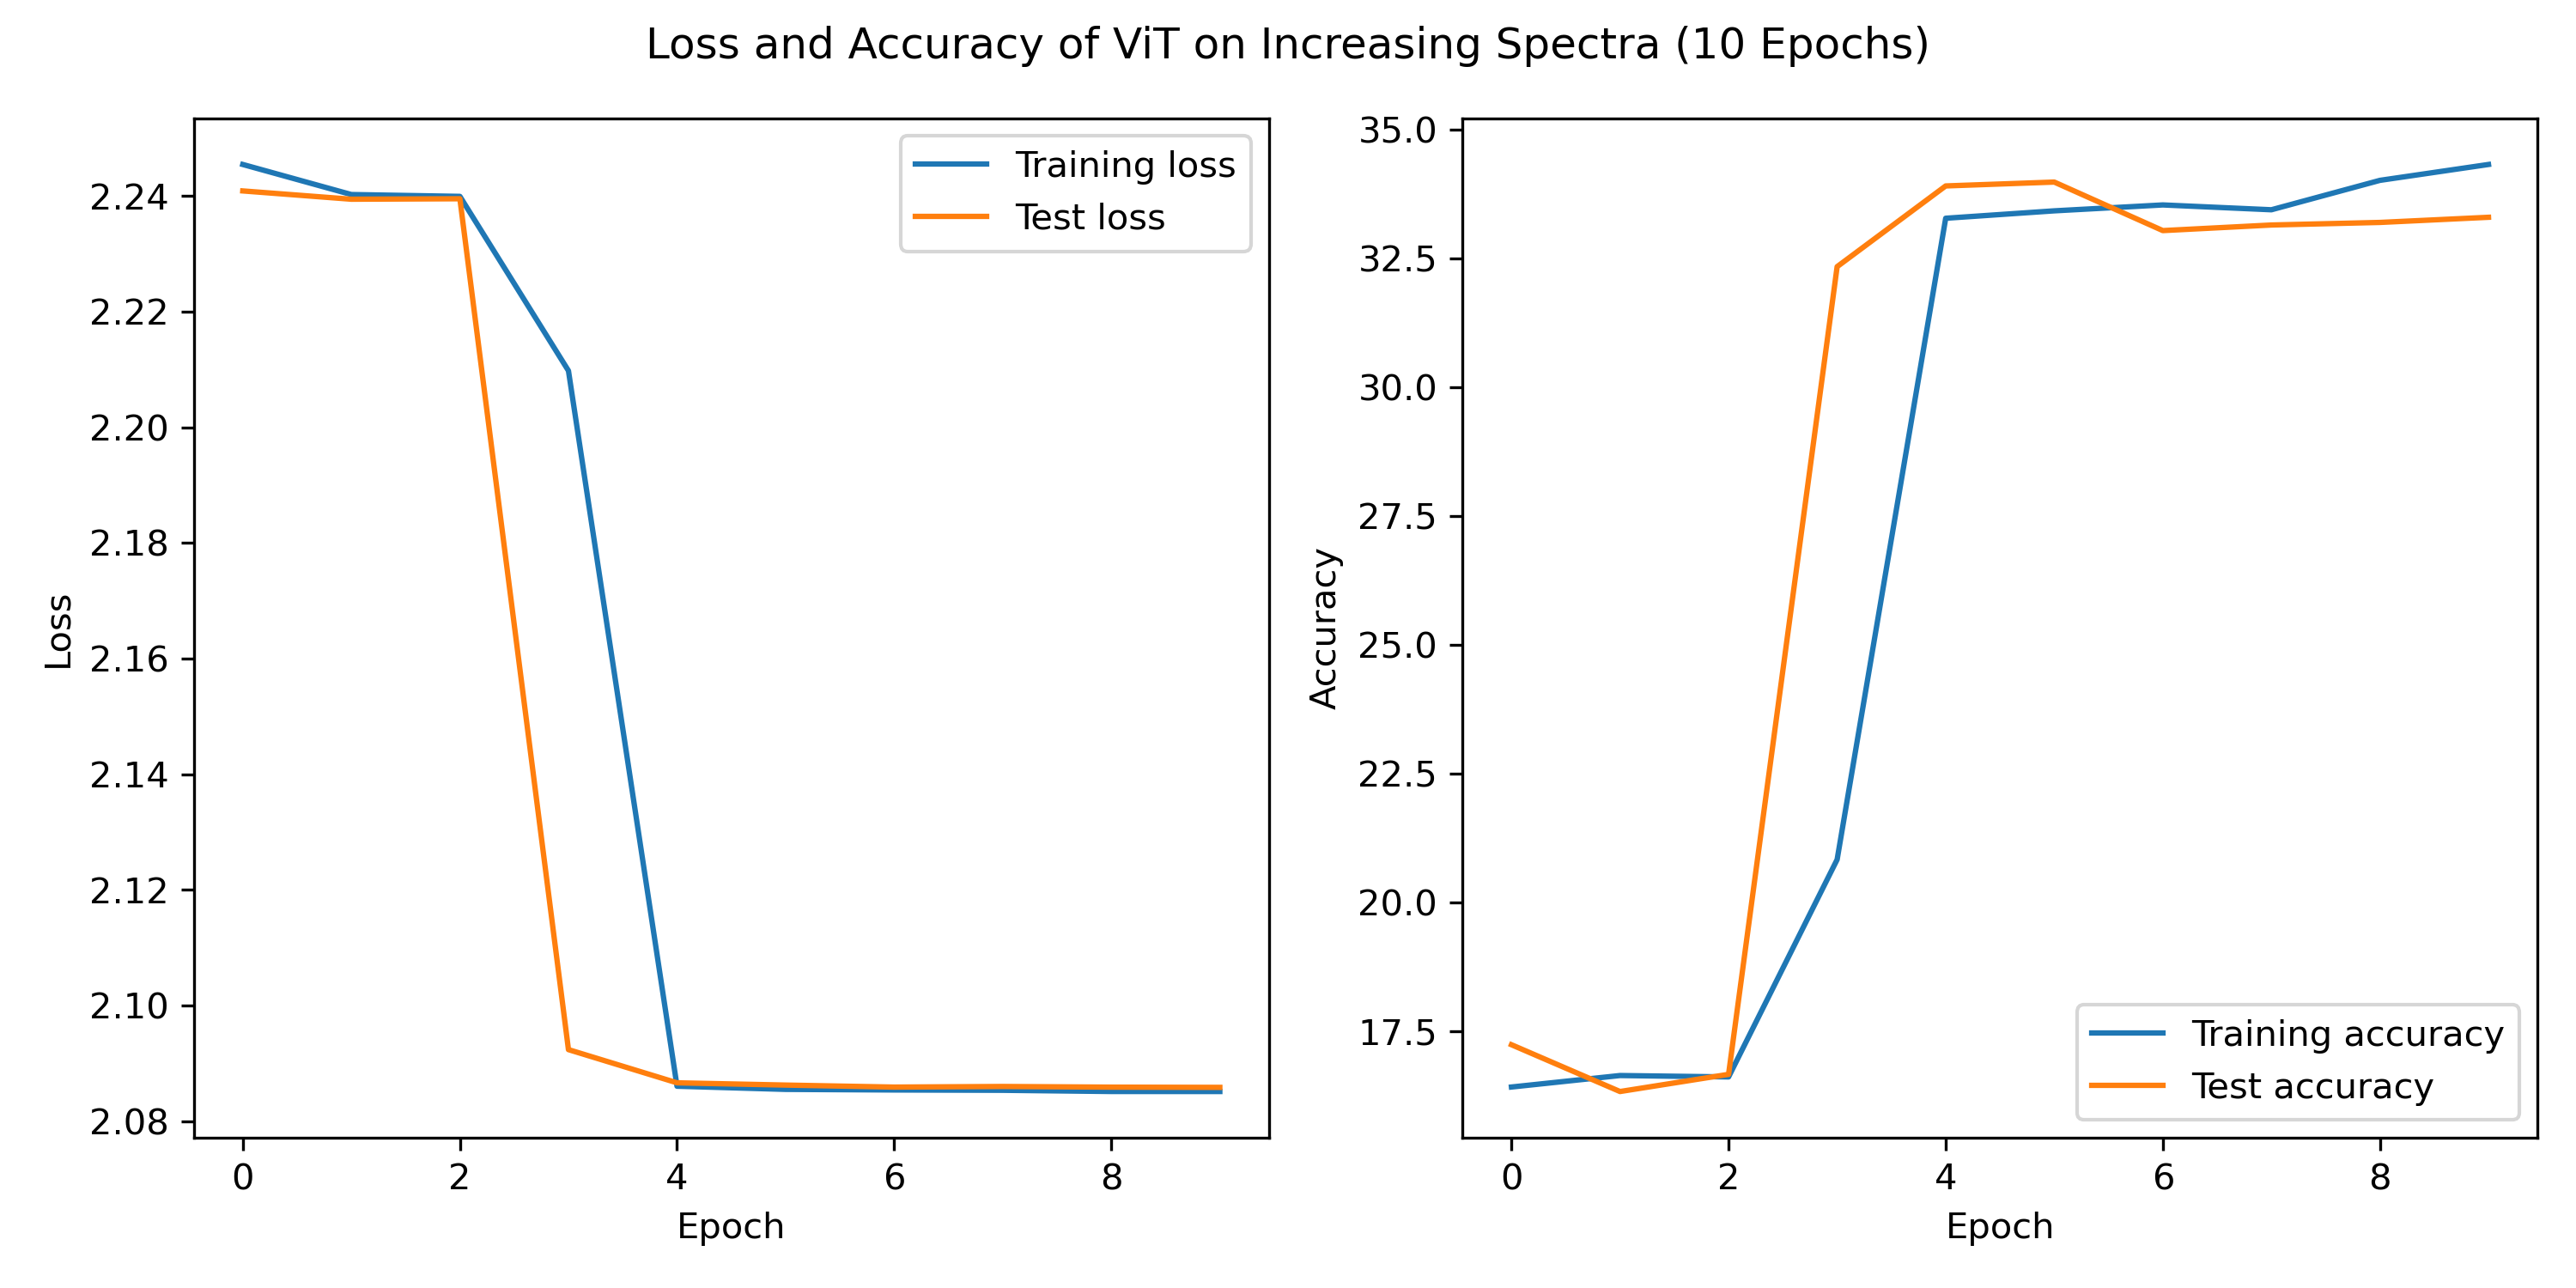
\includegraphics[width=11cm]{figures/pre_testing/SNR2_training_epoch.png}}
        \qquad
        \subfloat[\centering~SNR = 10\label{fig:snr10}]{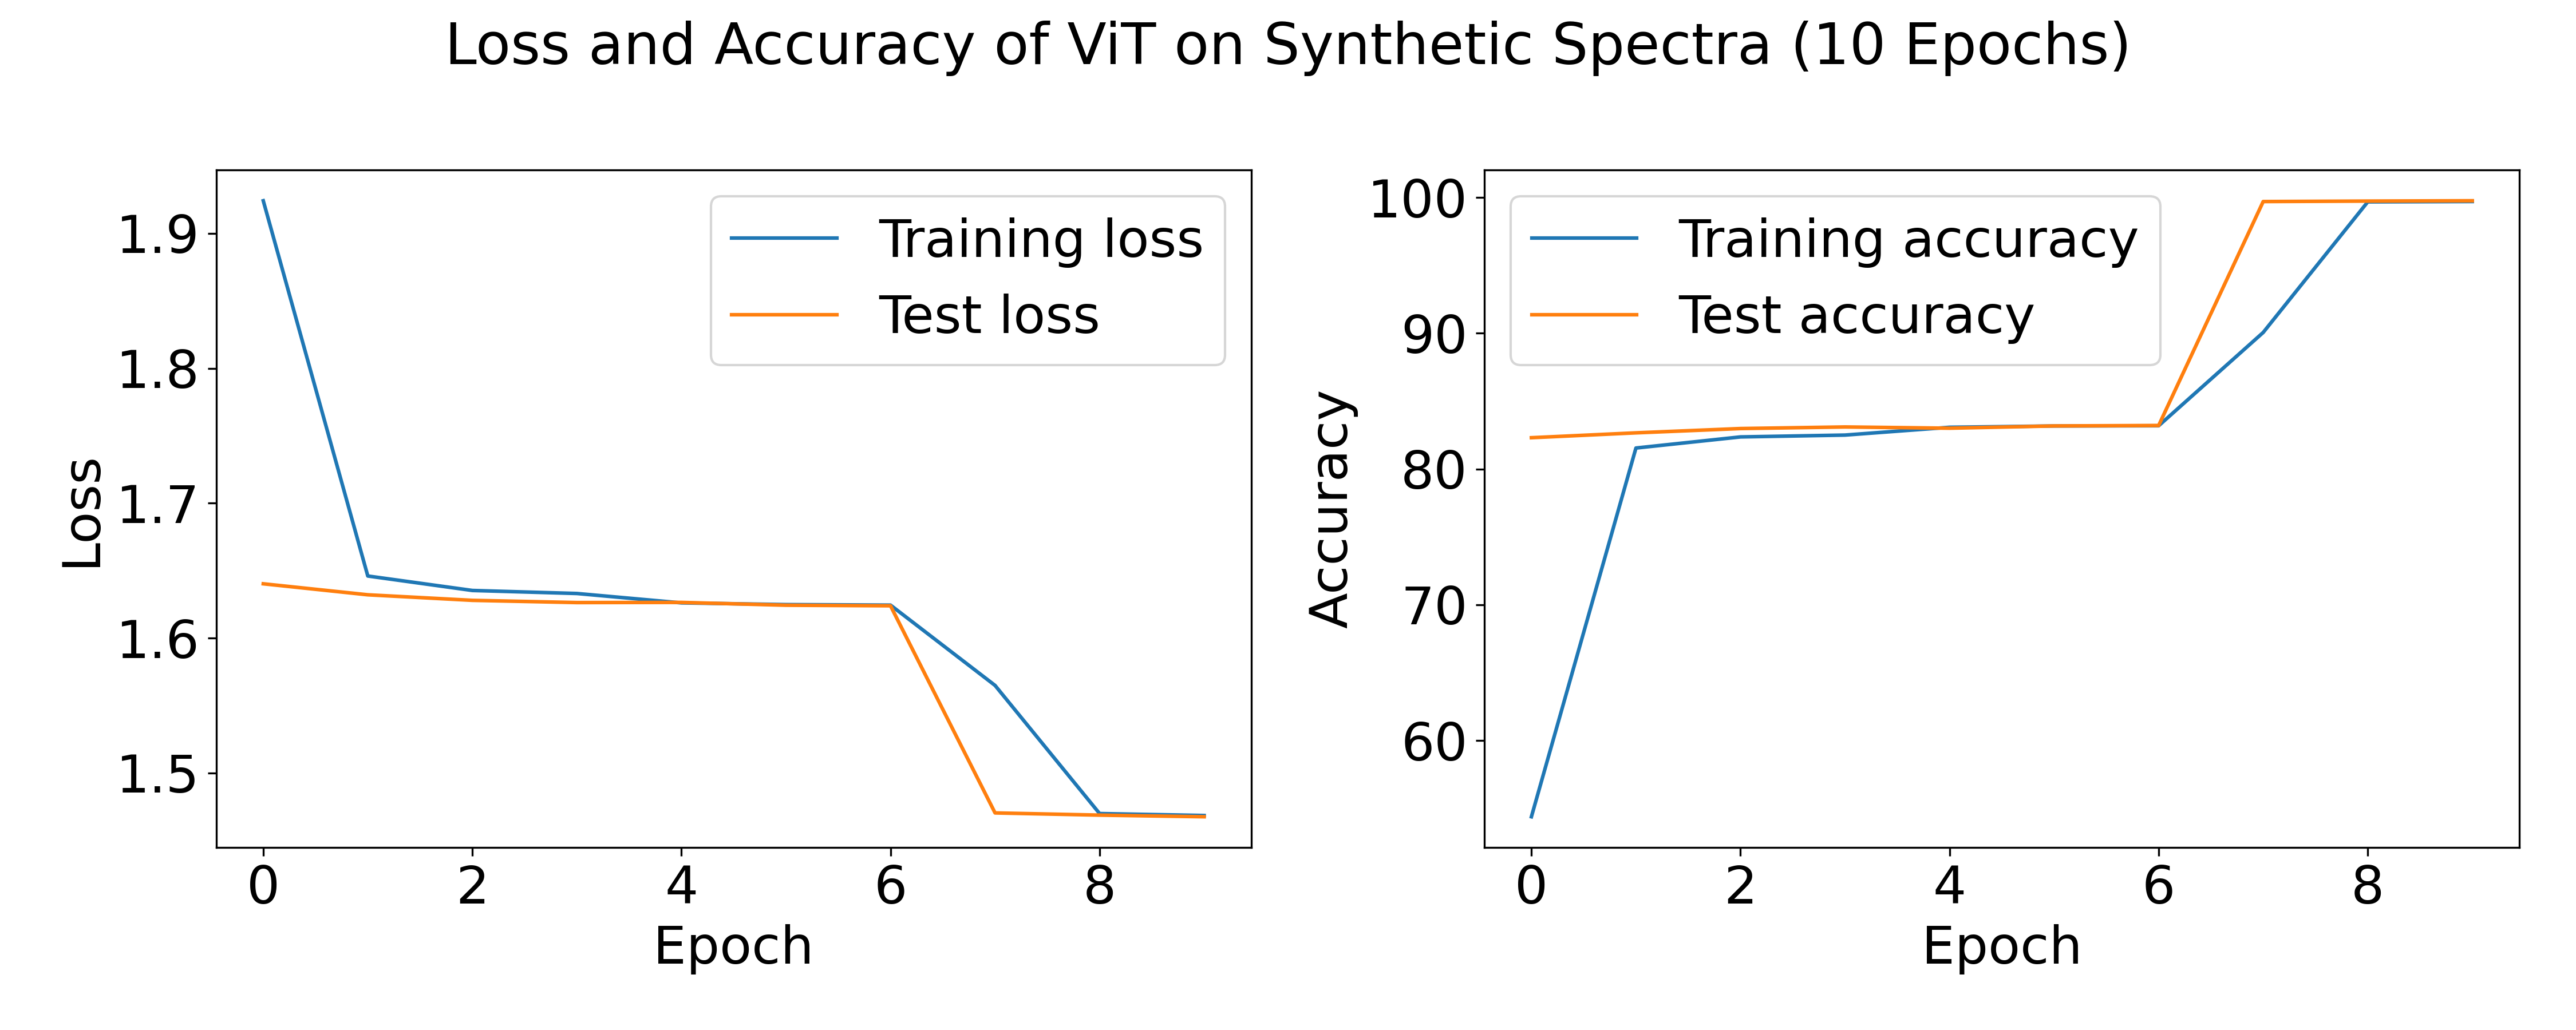
\includegraphics[width=11cm]{figures/pre_testing/SNR10_training_epoch.png}}
        \caption[Verification of ViT: Synthetic Dataset]{Training of Spectral ViT on synthetic datasets. The model was able to reach 100\% accuracy on the test set of SNR=10 (top), 
        but failed to reach an accuracy of 50\% on the test set of SNR=2 (bottom).}
    \label{fig:synth_spectra_training}
    \end{figure}
\end{frame}

%%%%%%%%%%%%%%%%%%%%%%%%%%%%%%%%%%%%%%%%%%%%%%%%%%%%%%%%%%%%%%%%%%%%%%%%
\begin{frame}
    \begin{figure}[t!]
        \centering
        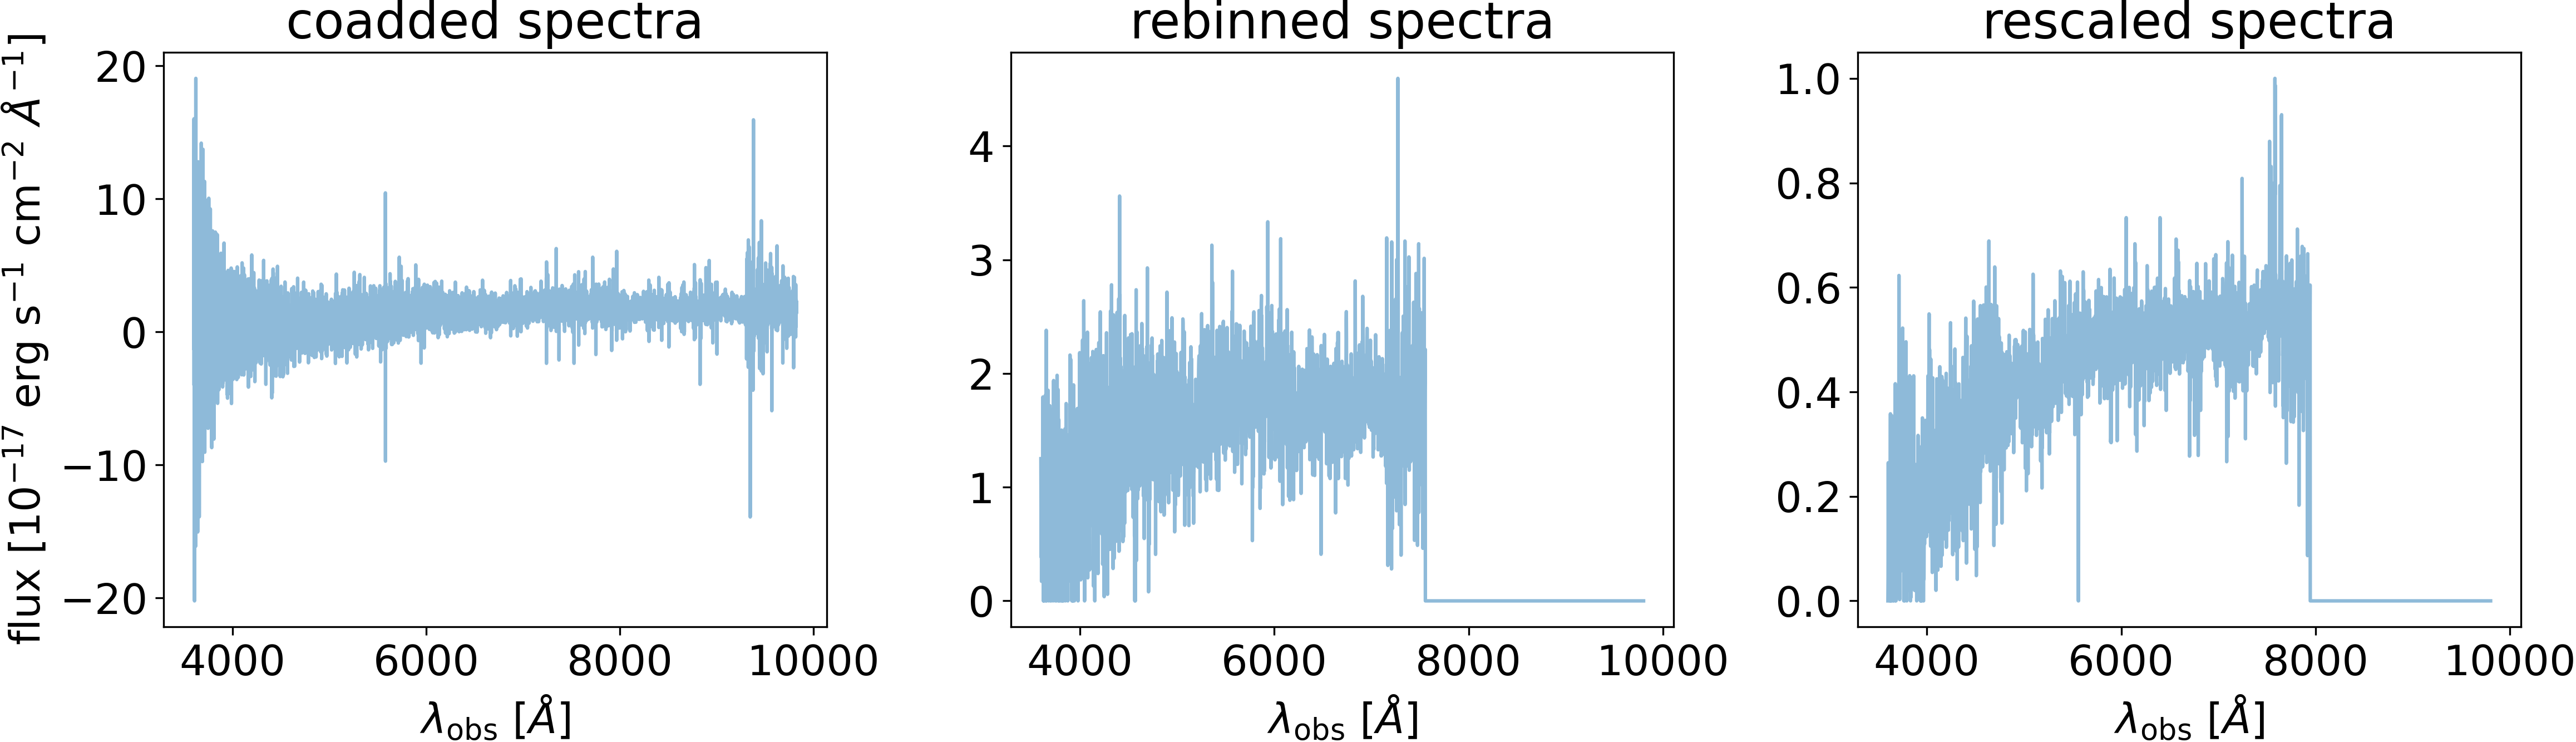
\includegraphics[width=\textwidth]{figures/preprocess/3600_Zcorrected_spectra.png}
        \caption{DESI Spectra Pre-Processing --  Redshift Corrected}
        % ]{DESI synthetic spectra undergoing pre-processing. The different bands
        % are first coadded together (left image). This is then  corrected to the galaxies rest frame and separated into 3600 
        % log-scale bins (center image). Finally, the sample is normalized between 0 and 1 (right image)}
        \label{fig:spectra_preproc}
%     \end{figure} 
% \end{frame}
%     \begin{figure}[b!]
%         \centering
        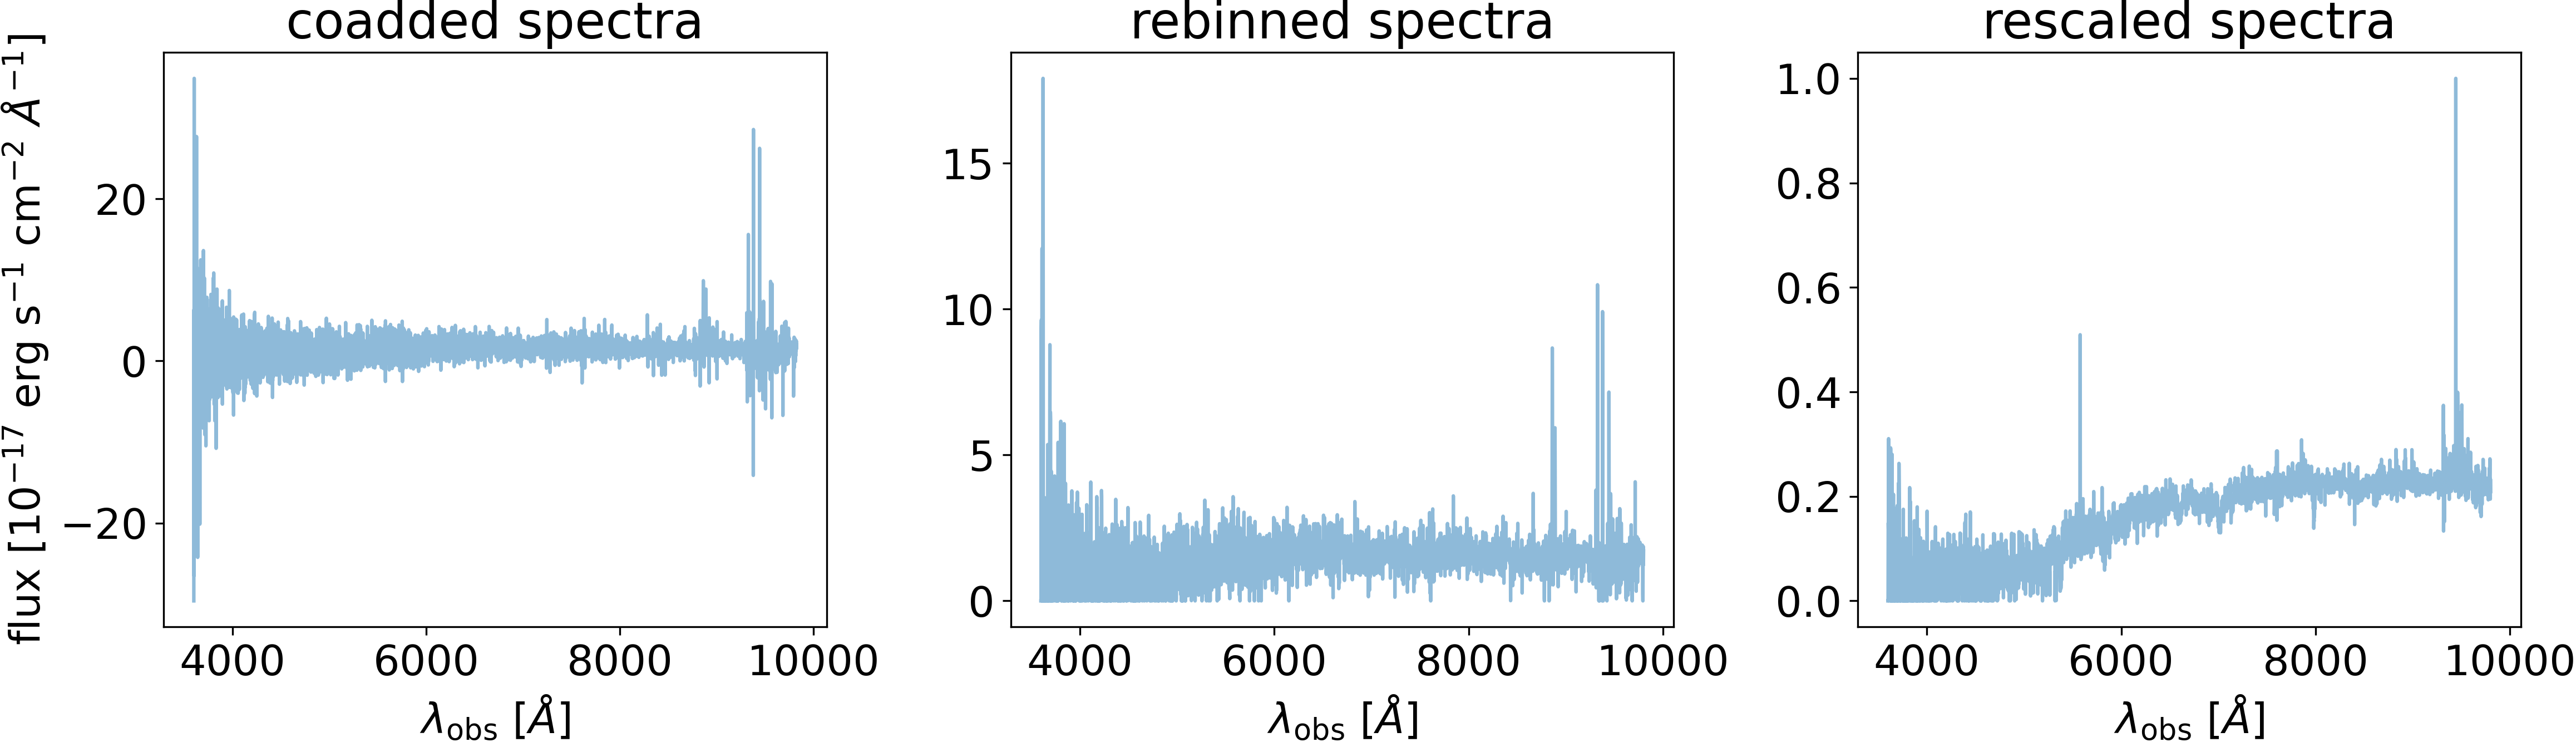
\includegraphics[width=\textwidth]{figures/preprocess/3600_Zrestframe_spectra.png}
        \caption{DESI Spectra Pre-Processing --  Non-Redshift Corrected}
        % \caption[Spectra Pre-Processing -- Not Redshift Corrected]{DESI synthetic spectra undergoing pre-processing. 
        % The different bands are first coadded together (left image). This is then separated 
        % into 3600 log-scale bins without any redshift correction (center image). Finally, 
        % the sample is normalized between 0 and 1 (right image)}
        \label{fig:sepctra_preproc_nored}
    \end{figure} 
\end{frame}

%%%%%%%%%%%%%%%%%%%%%%%%%%%%%%%%%%%%%%%%%%%%%%%%%%%%%%%%%%%%%%%%%%%%%%%%
\begin{frame}
    \begin{table}[t!]
        \small
        \centering
        \sffamily
        \begin{tabular}{lc}
	\toprule
    \textbf{Hyperparameter} & \textbf{Value} \\
    \midrule
    Learning Rate & 0.00004135238172950965 \\ 
    \midrule
    Regularization & 0.06 \\ 
    \midrule
    Dropout Rate & 0.40904759925886294\\
    \midrule
    Batch Size & 50 \\
    \bottomrule
\end{tabular}

        \caption{Hyperparameters of the CNN used to classify DESI spectra. CNN adapted 
        from \textcite{Sepeku2022}.}
        \label{tab:cnn_hyperparameters}
    \end{table}
    \begin{figure}[b!]
        \centering
        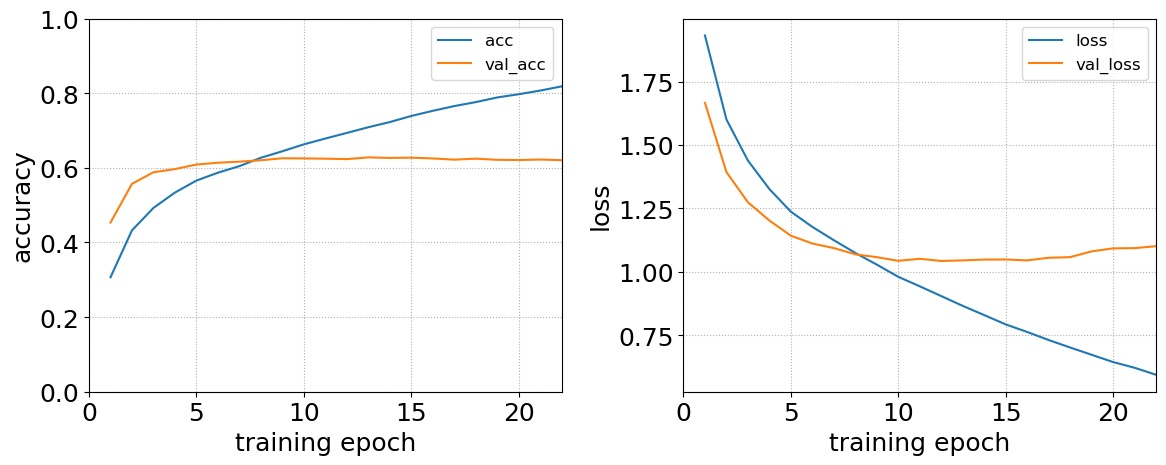
\includegraphics[width=.85\linewidth]{figures/cnn/cnn_training_history.jpg}
        \caption[CNN Training]{Training of the CNN on synthetic DESI spectra.}
        \label{fig:cnn_training}
    \end{figure}
\end{frame}


%%%%%%%%%%%%%%%%%%%%%%%%%%%%%%%%%%%%%%%%%%%%%%%%%%%%%%%%%%%%%%%%%%%%%%%%
\begin{frame}
    \begin{table}[t!]
        \small
        \centering
        \sffamily
        \begin{tabular}{lcc}
	\toprule
    \textbf{Hyperparameter} & \textbf{Smaller Architecture} & \textbf{Larger Architecture} \\
    \midrule
    Learning Rate & 0.0001 & 0.01 \\ 
    \midrule
    Batch Size & 16 & 16 \\
    \midrule
    Blocks & 4 & 4 \\
    Heads & 5 & 12 \\
    Hidden Dimension & 25 & 72 \\
    \bottomrule
\end{tabular}

        \caption{Hyperparameters of the smaller and larger Spectral ViT architecture used to classify DESI spectra.}
        \label{tab:t_hyper}
    \end{table}
    
    \begin{figure}[b!]
        \centering
        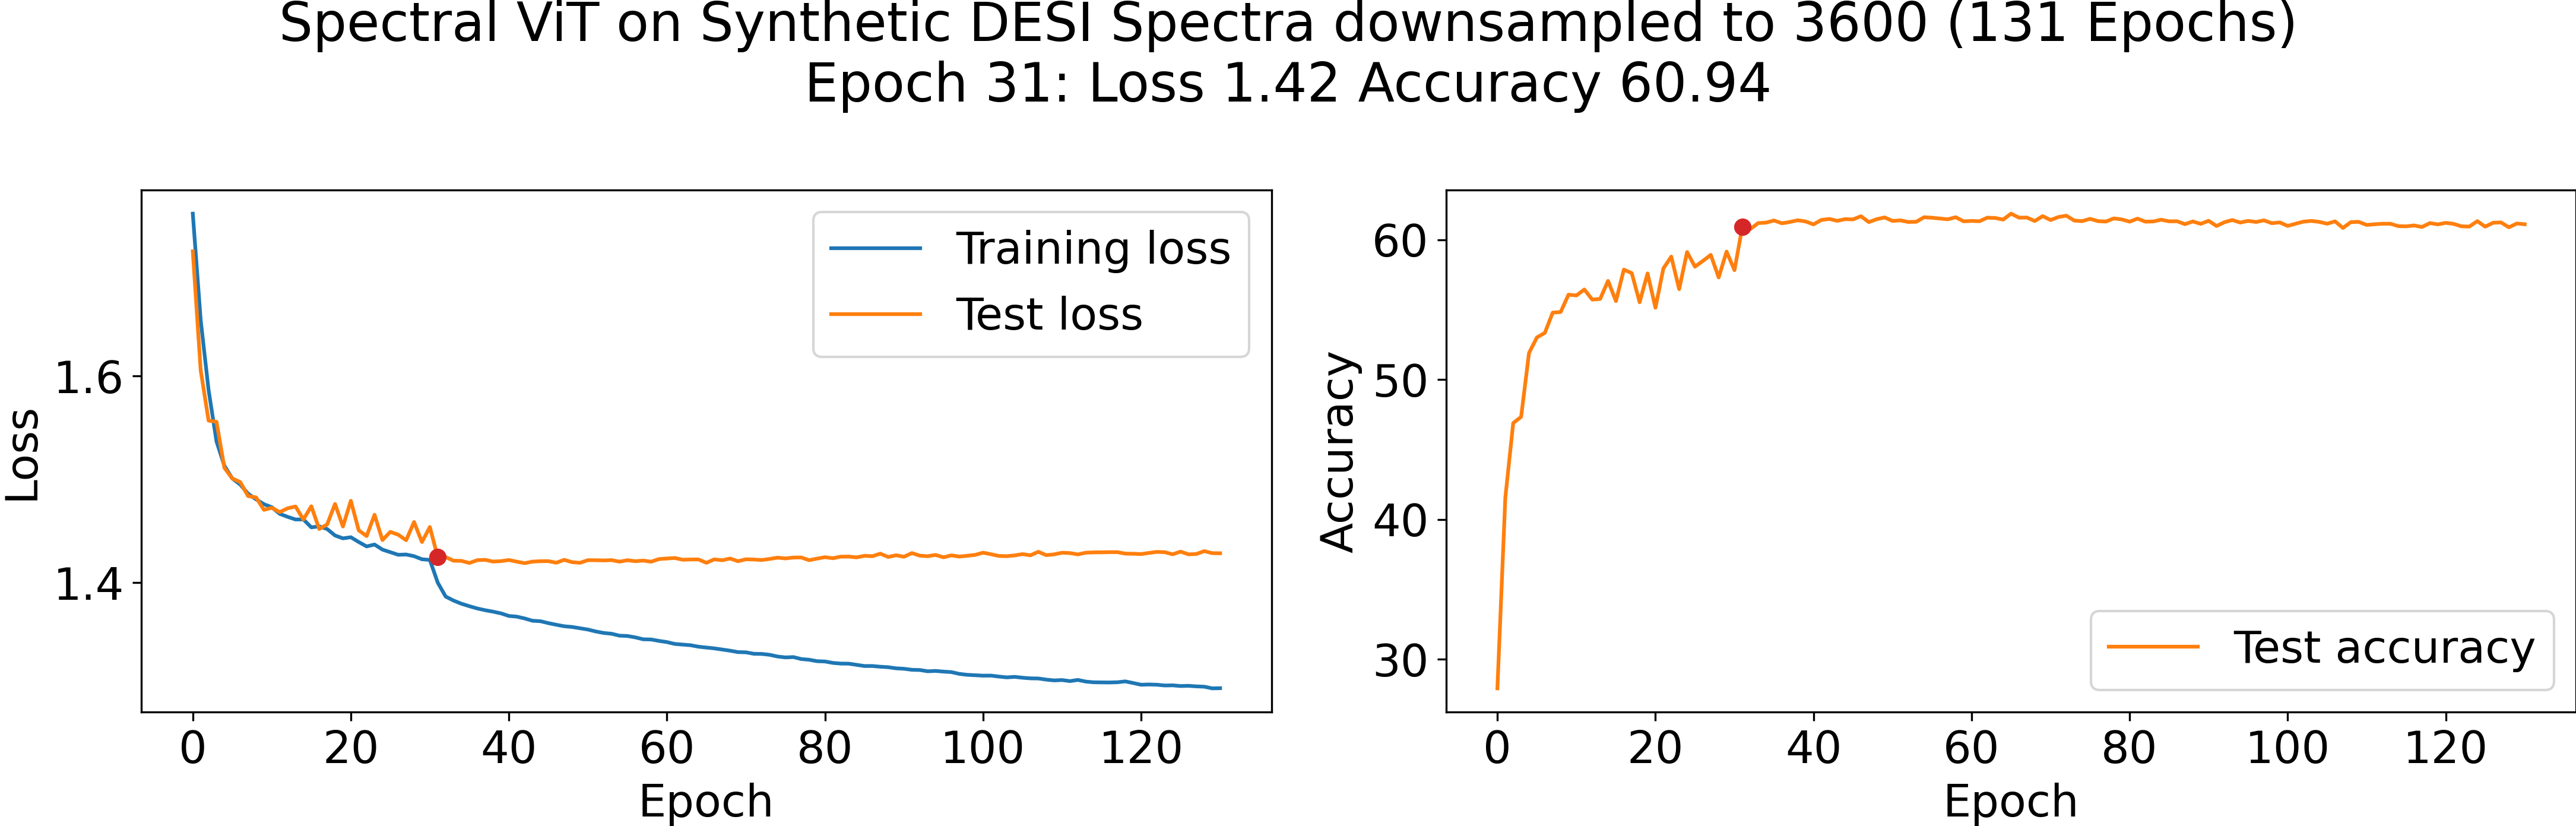
\includegraphics[width=.85\linewidth]{figures/v1_real/vit_model_V1_original_redotraining_new.png}
        \caption{Training of Spectral ViT: V1}
        % {Training of the small architecture on redshift-corrected spectra downsampled to 3600 bins. Over-fitting was determined to have occurred by Epoch 31.}
        \label{fig:vit1_training}
    \end{figure}
\end{frame}


%%%%%%%%%%%%%%%%%%%%%%%%%%%%%%%%%%%%%%%%%%%%%%%%%%%%%%%%%%%%%%%%%%%%%%%%

\begin{frame}{Additional (Failed) Training}
\centering
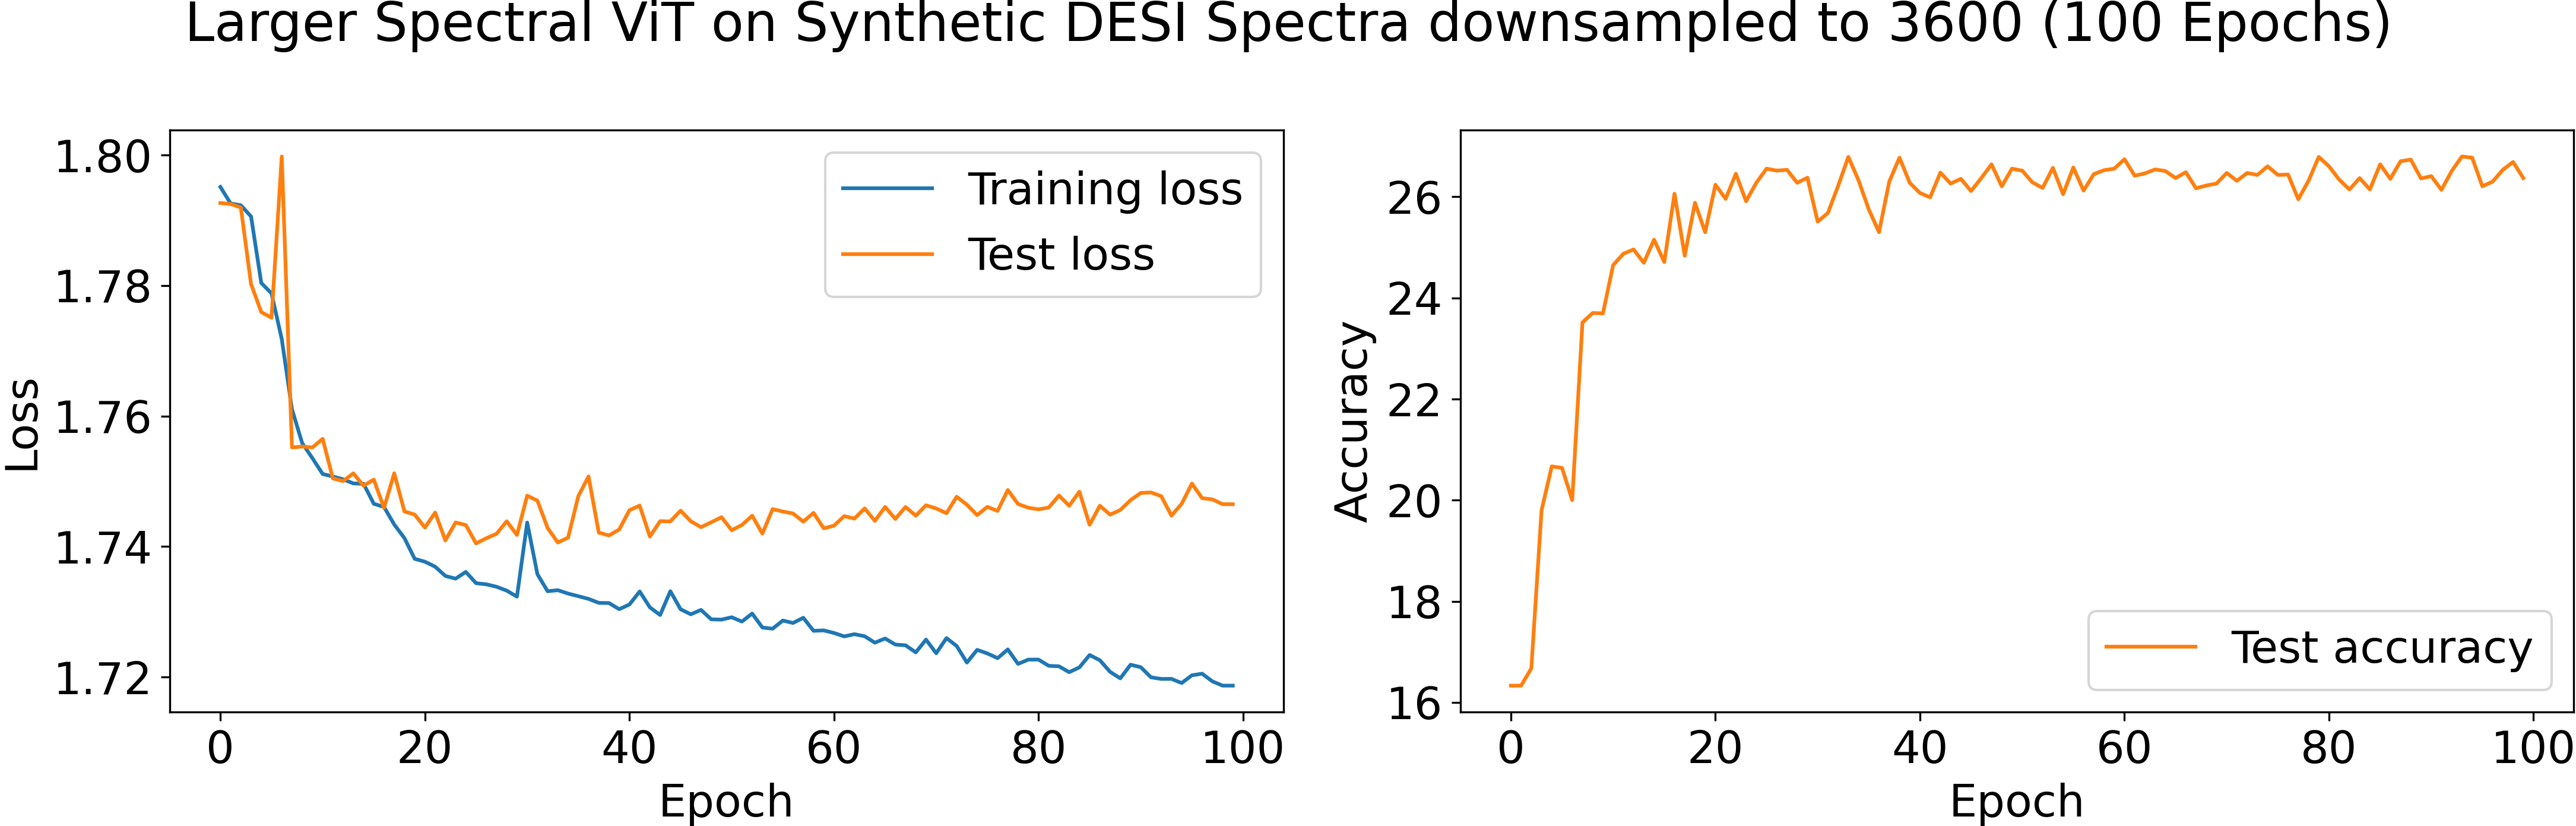
\includegraphics[width=5.5cm]{figures/v1_real/vit_model_V1_bigtraining_new.png}\\
\begin{columns}[t]
\column{.5\textwidth}
\centering
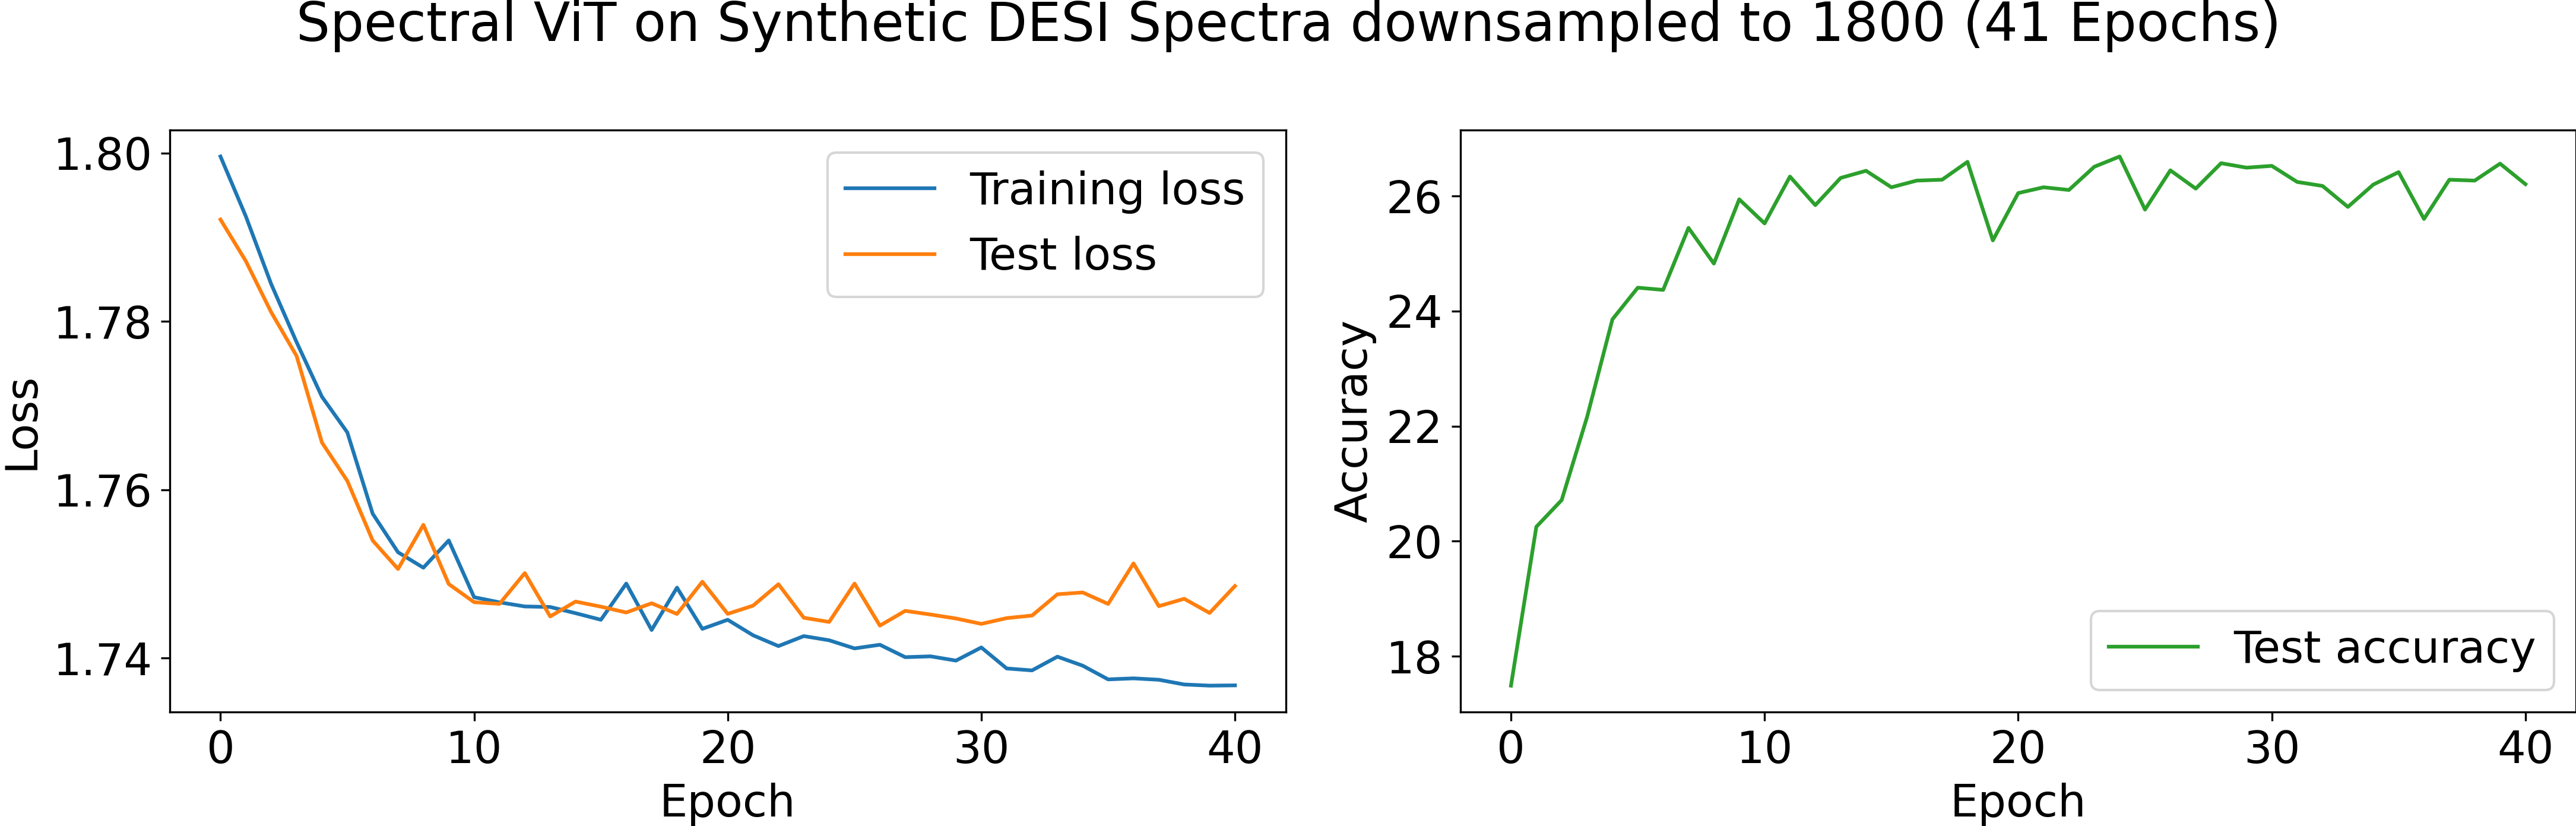
\includegraphics[width=5.5cm]{figures/vit_model_V1.2training_new.png}
\column{.5\textwidth}
\centering
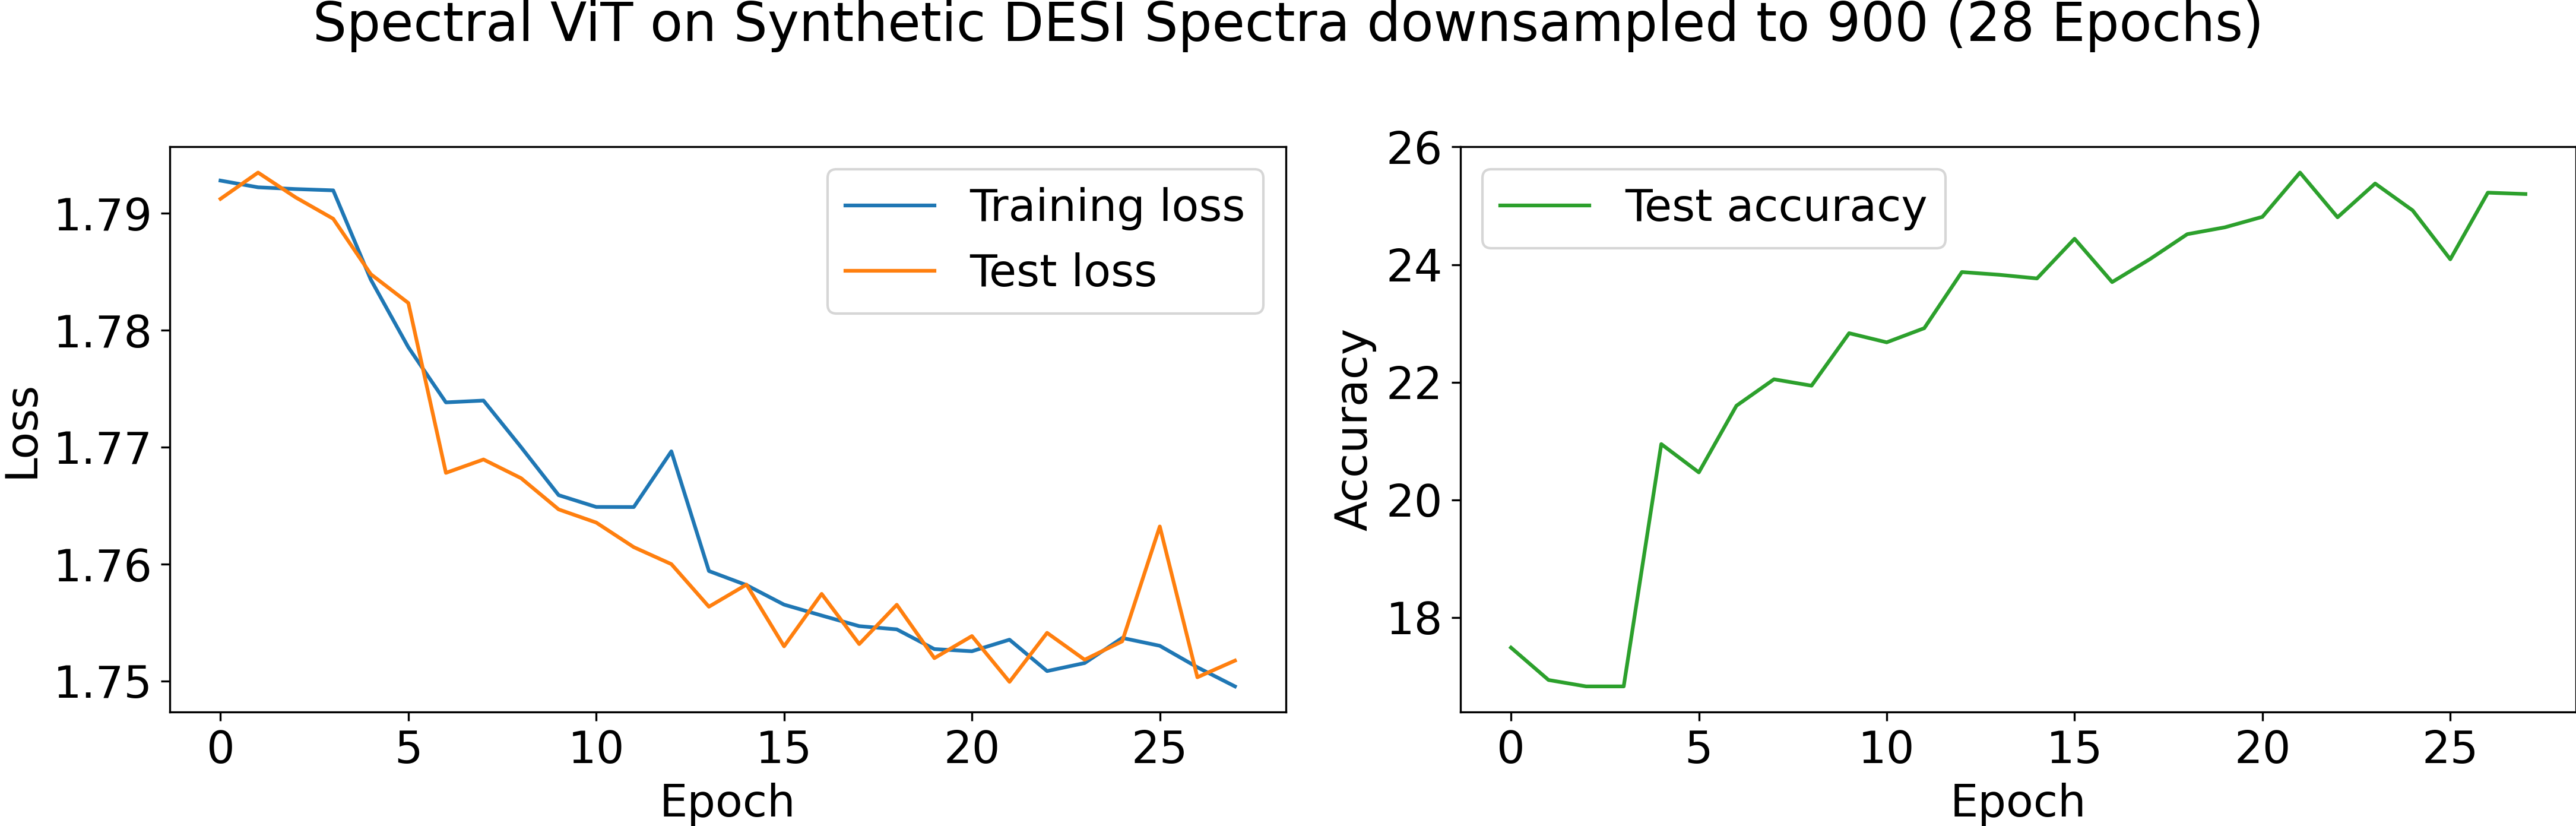
\includegraphics[width=5.5cm]{figures/vit_model_V1.3_muchsmallermodeltraining_new.png}\\
\end{columns}
\end{frame}


\begin{frame}{Training for Non-Redshift Corrected Data}
\centering
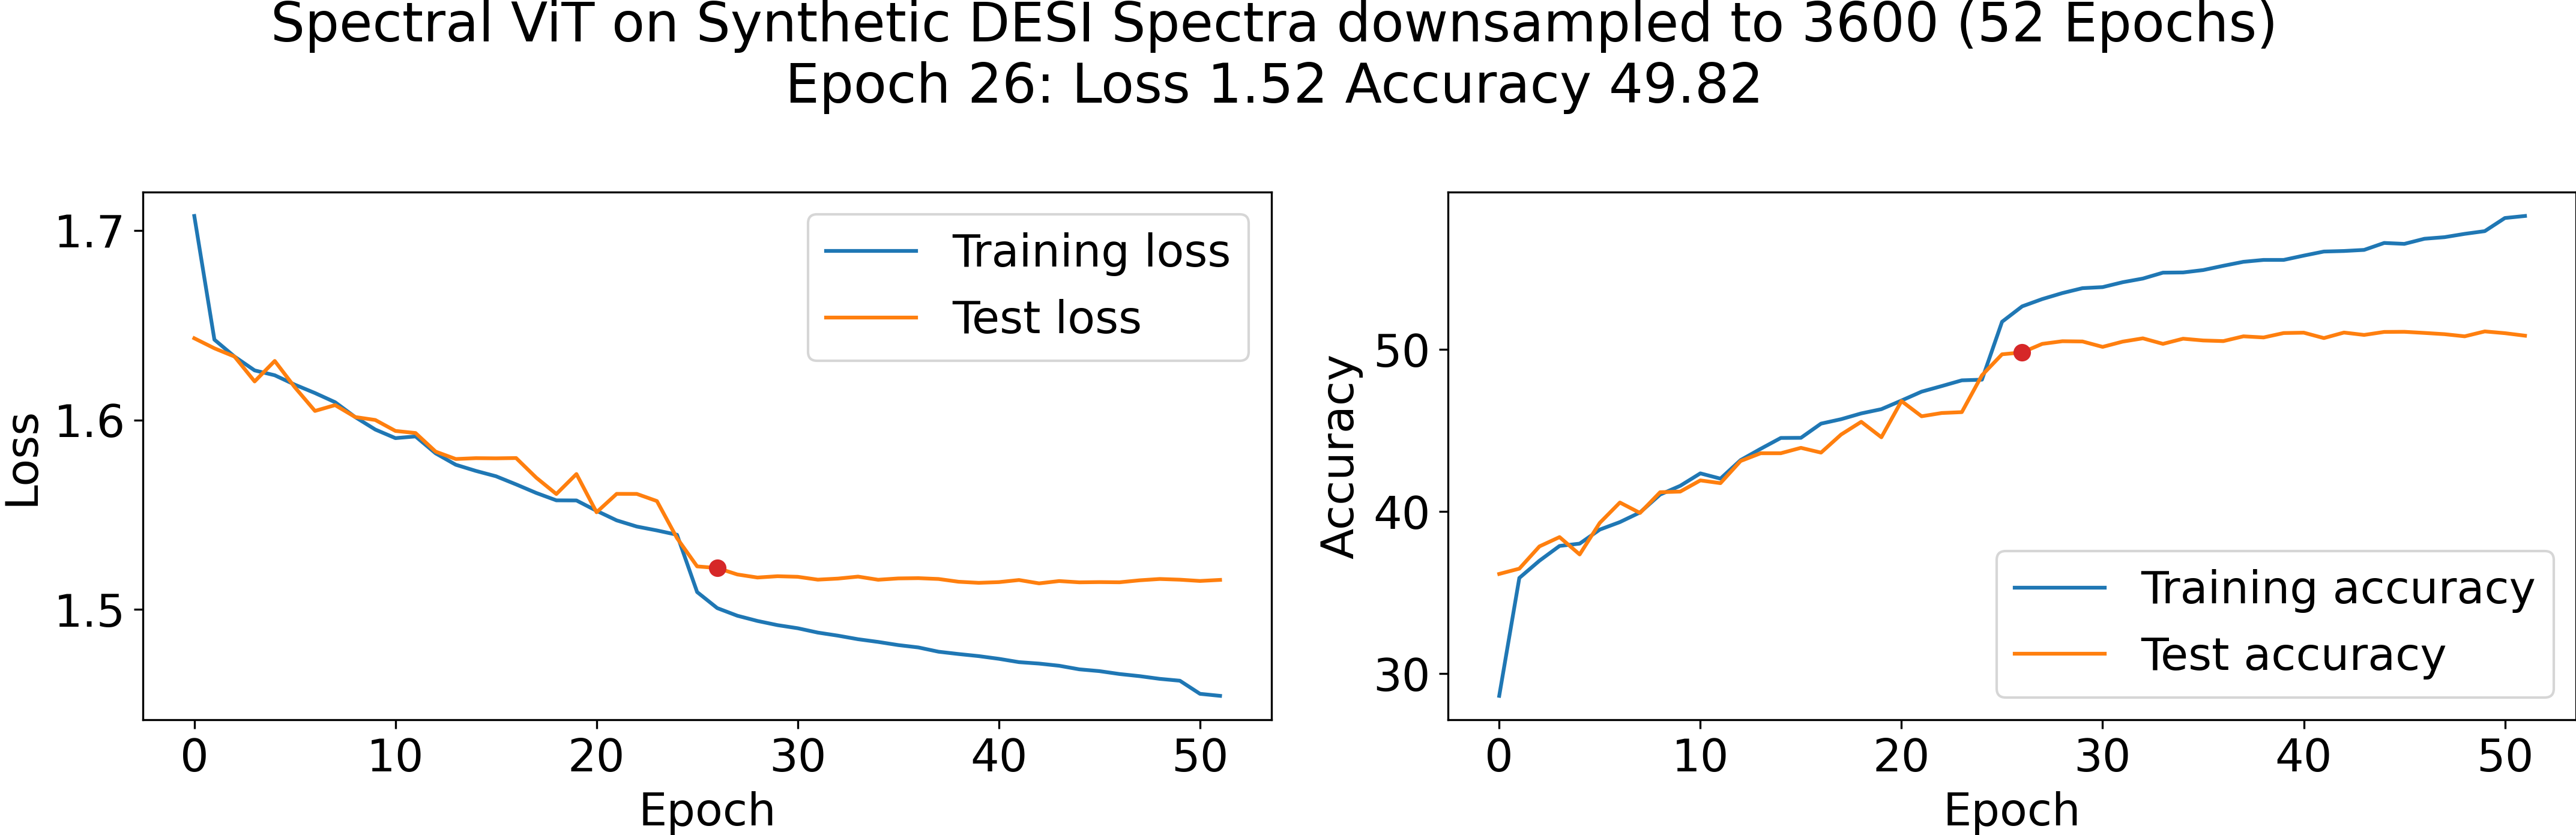
\includegraphics[width=.85\linewidth]{figures/v2_real/vit_model_V2training_new.png}
\end{frame}


\begin{comment}
%%%%%%%%%%%%%%%%%%%%%%%%%%%%%%%%%%%%%%%%%%%%%%%%%%%%%%%%%%%%%%%%%%%%%%%%
\begin{frame}
    \begin{figure}[t!]
        \centering
        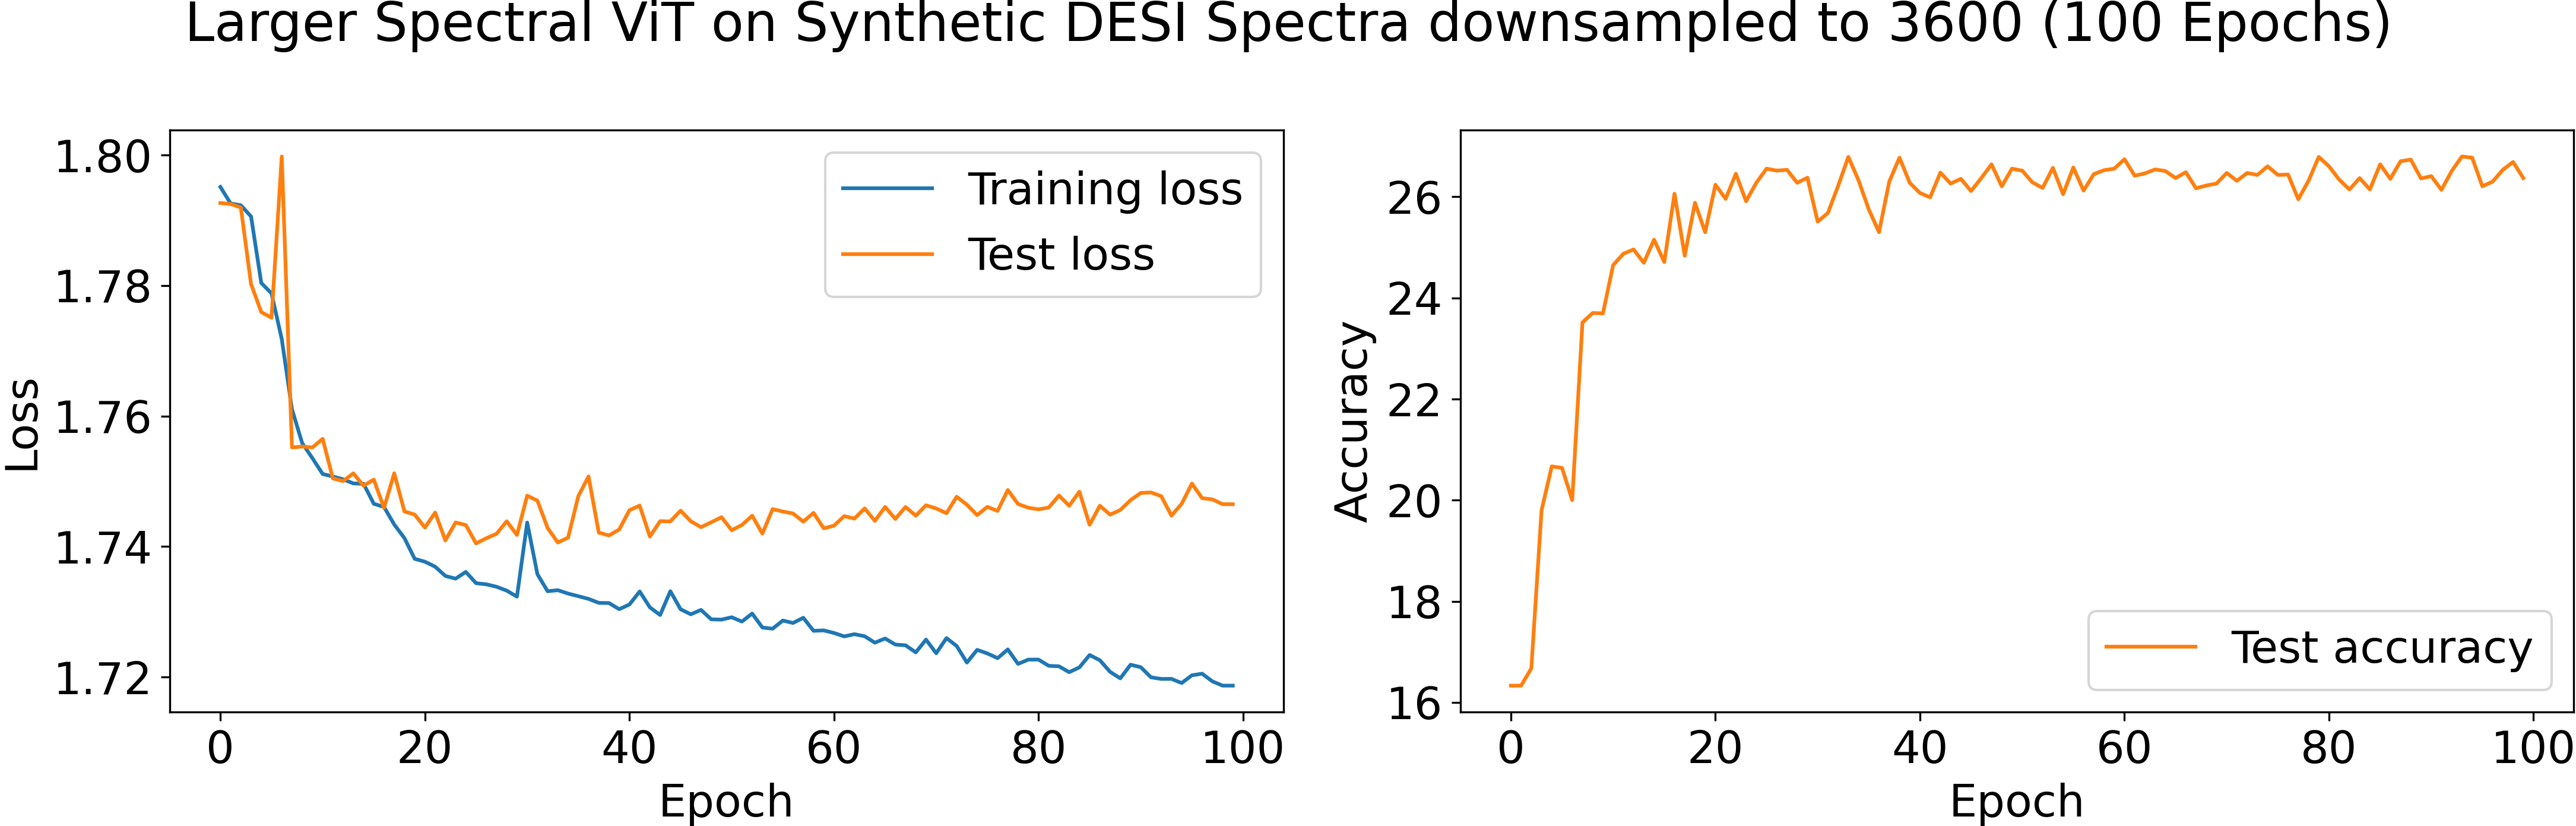
\includegraphics[width=.85\linewidth]{figures/v1_real/vit_model_V1_bigtraining_new.png}
        \caption[Training of Spectral ViT: V1 Big]{Training of the large architecture on Redshift-corrected spectra downsampled to 3600 bins. No convergence above random guessing was observed. }
        \label{fig:vit1_big_training}
    \end{figure}
\end{frame}

%%%%%%%%%%%%%%%%%%%%%%%%%%%%%%%%%%%%%%%%%%%%%%%%%%%%%%%%%%%%%%%%%%%%%%%%
\begin{frame}
    \begin{figure}[hb!]
        \centering
        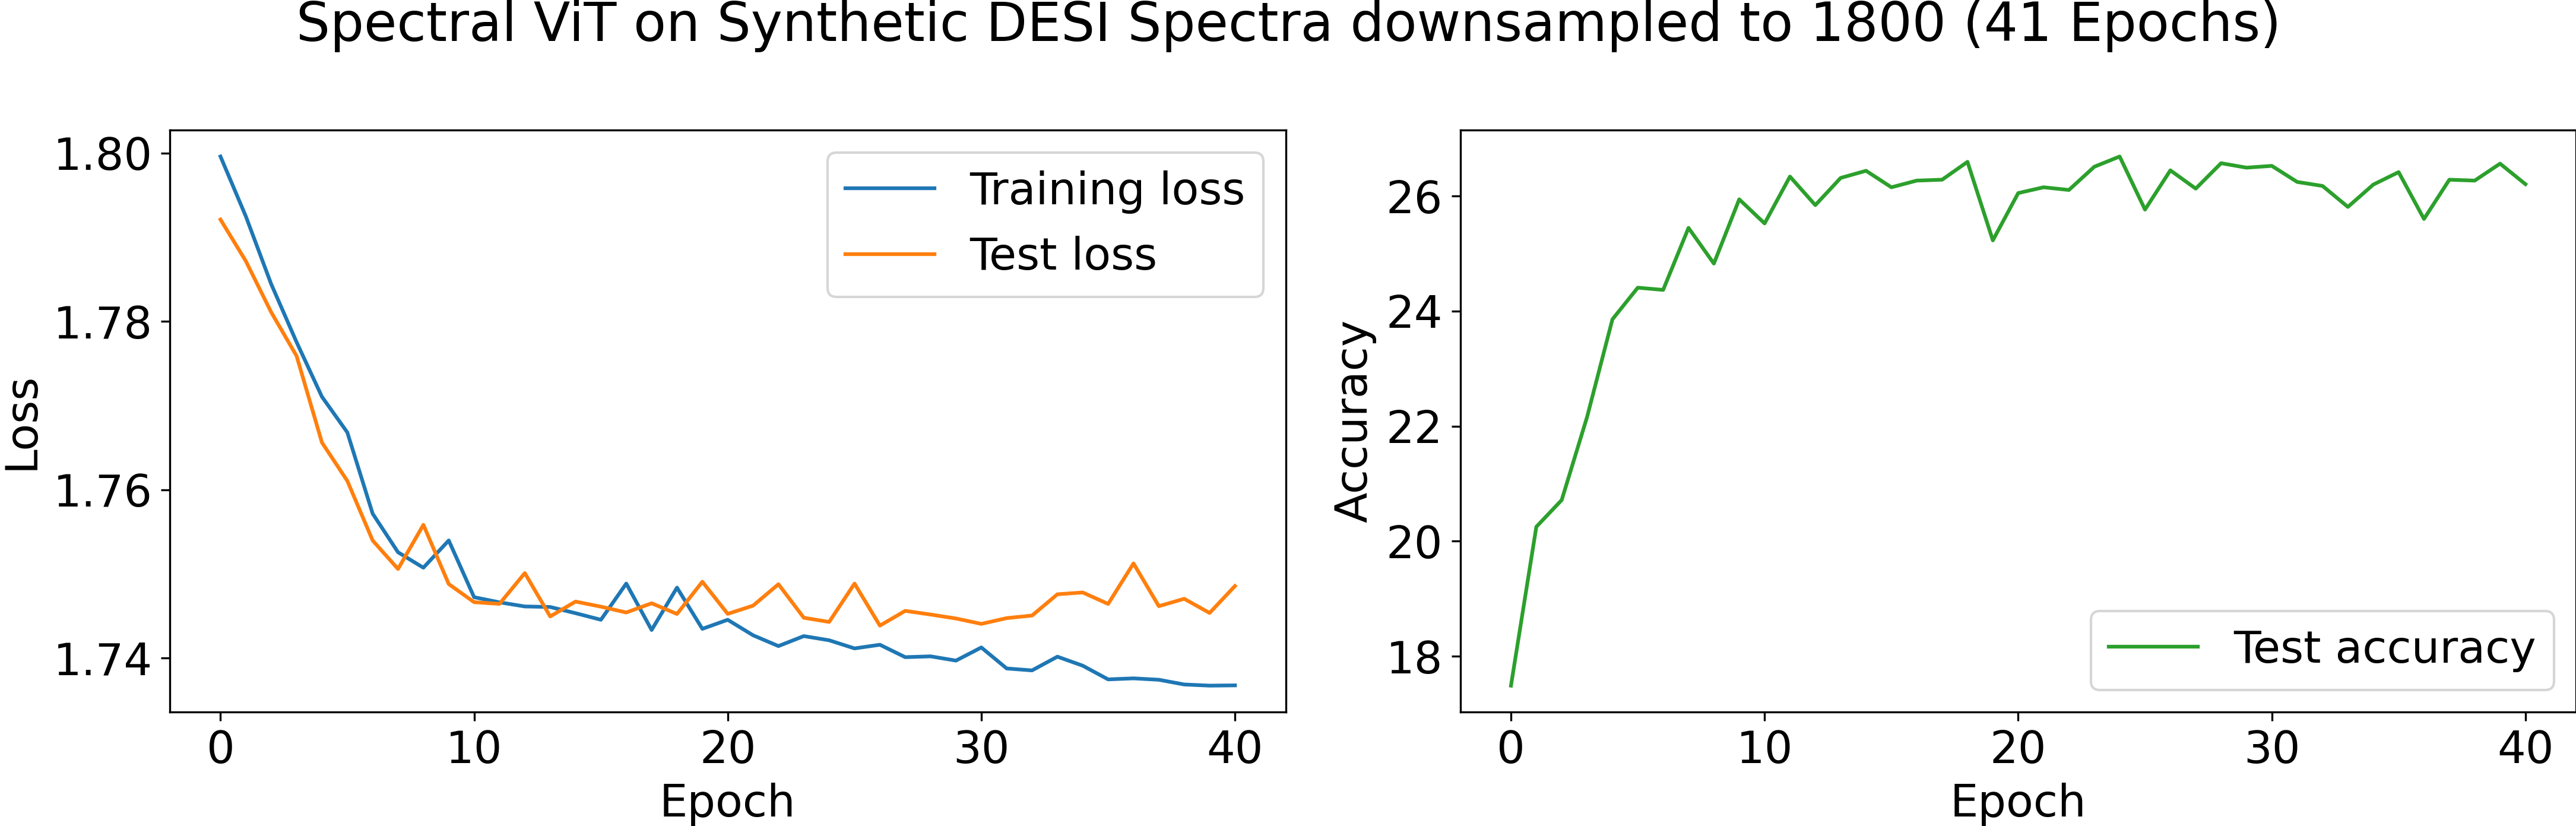
\includegraphics[width=.85\linewidth]{figures/vit_model_V1.2training_new.png}
        \caption[Training of Spectral ViT: V1.2]{Training of the small architecture on Redshift-corrected spectra downsampled to 1800 bins. No convergence above random guessing was observed. }
        \label{fig:vit1.2_training}
    \end{figure}
\end{frame}

%%%%%%%%%%%%%%%%%%%%%%%%%%%%%%%%%%%%%%%%%%%%%%%%%%%%%%%%%%%%%%%%%%%%%%%%
\begin{frame}
    \begin{figure}[t!]
        \centering
        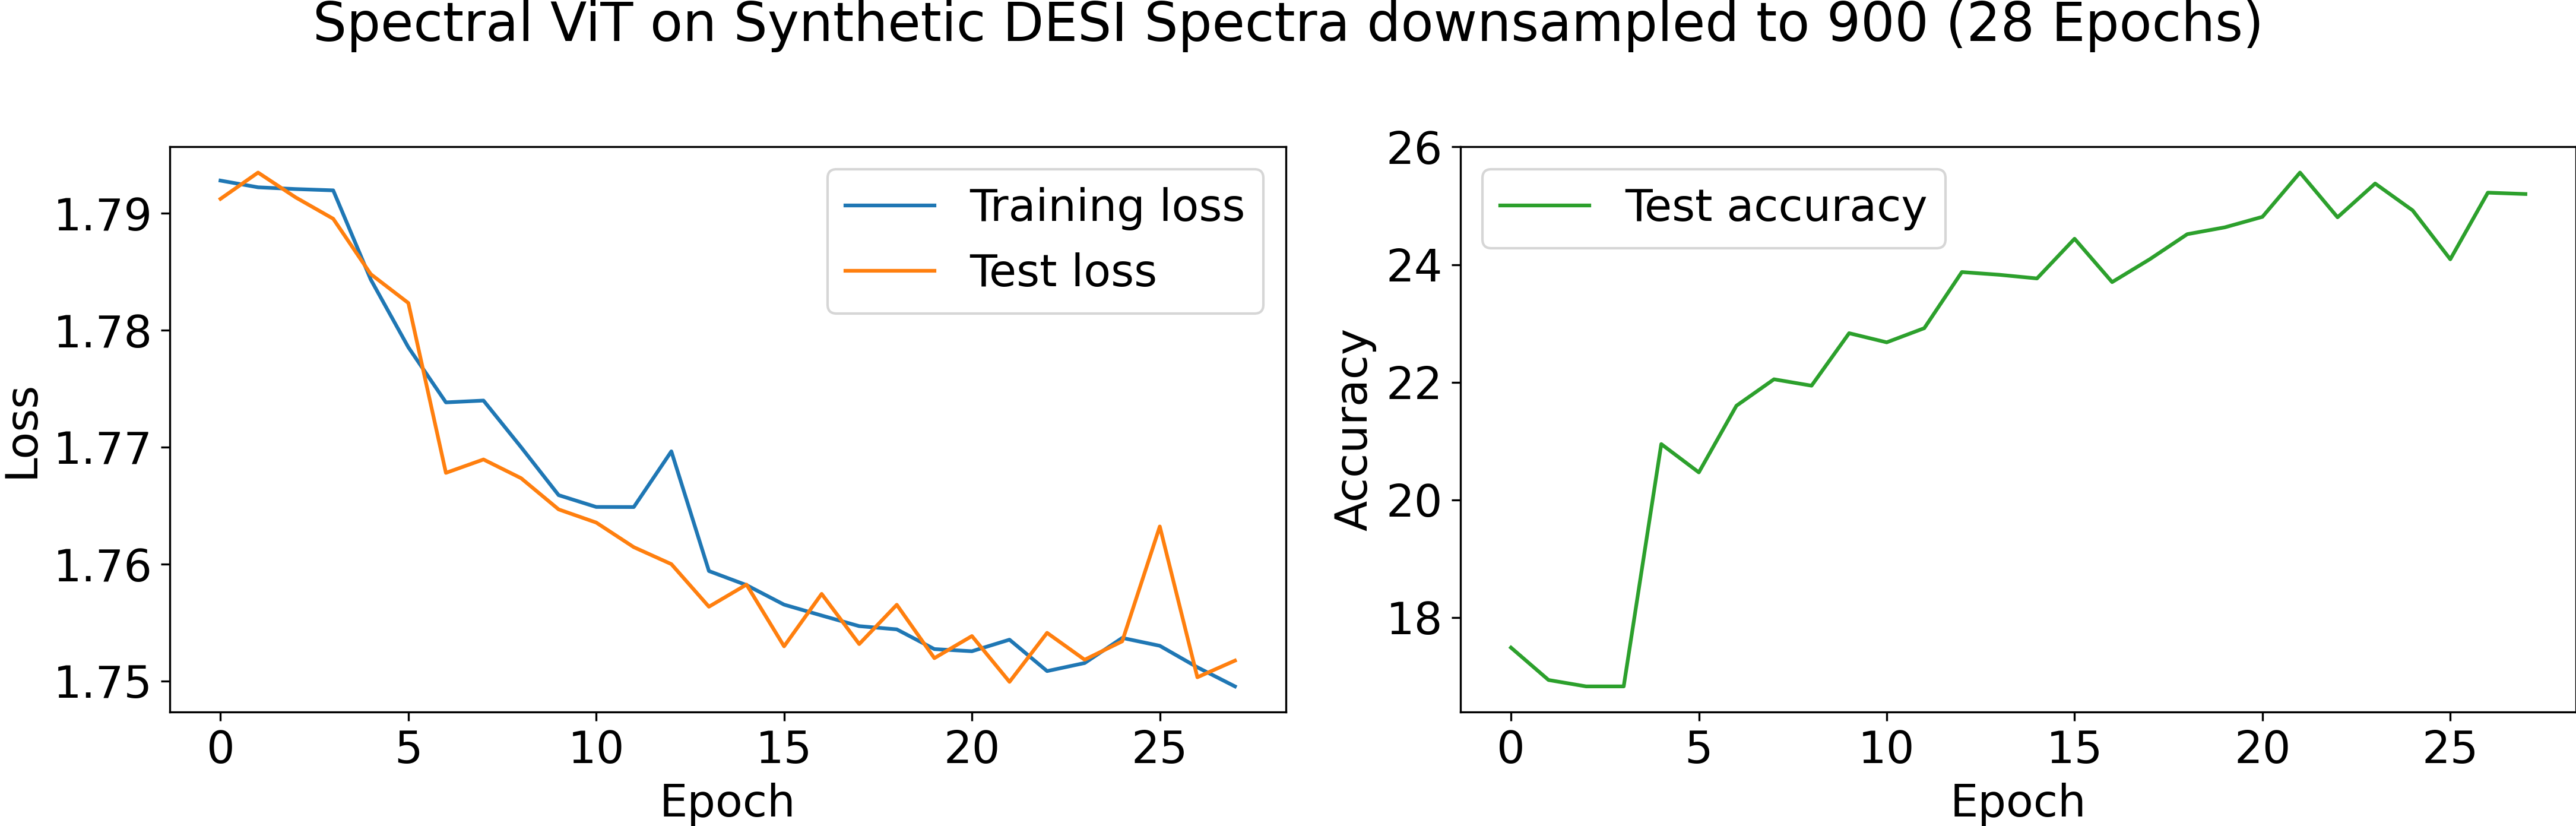
\includegraphics[width=.85\linewidth]{figures/vit_model_V1.3_muchsmallermodeltraining_new.png}
        \caption[Training of Spectral ViT: V1.3]{Training of the small architecture on Redshift-corrected spectra downsampled to 900 bins. No convergence above random guessing was observed. }
        \label{fig:vit1.3_training}
    \end{figure}
\end{frame}


%%%%%%%%%%%%%%%%%%%%%%%%%%%%%%%%%%%%%%%%%%%%%%%%%%%%%%%%%%%%%%%%%%%%%%%%
\begin{frame}
    \begin{figure}[t!]
        \centering
        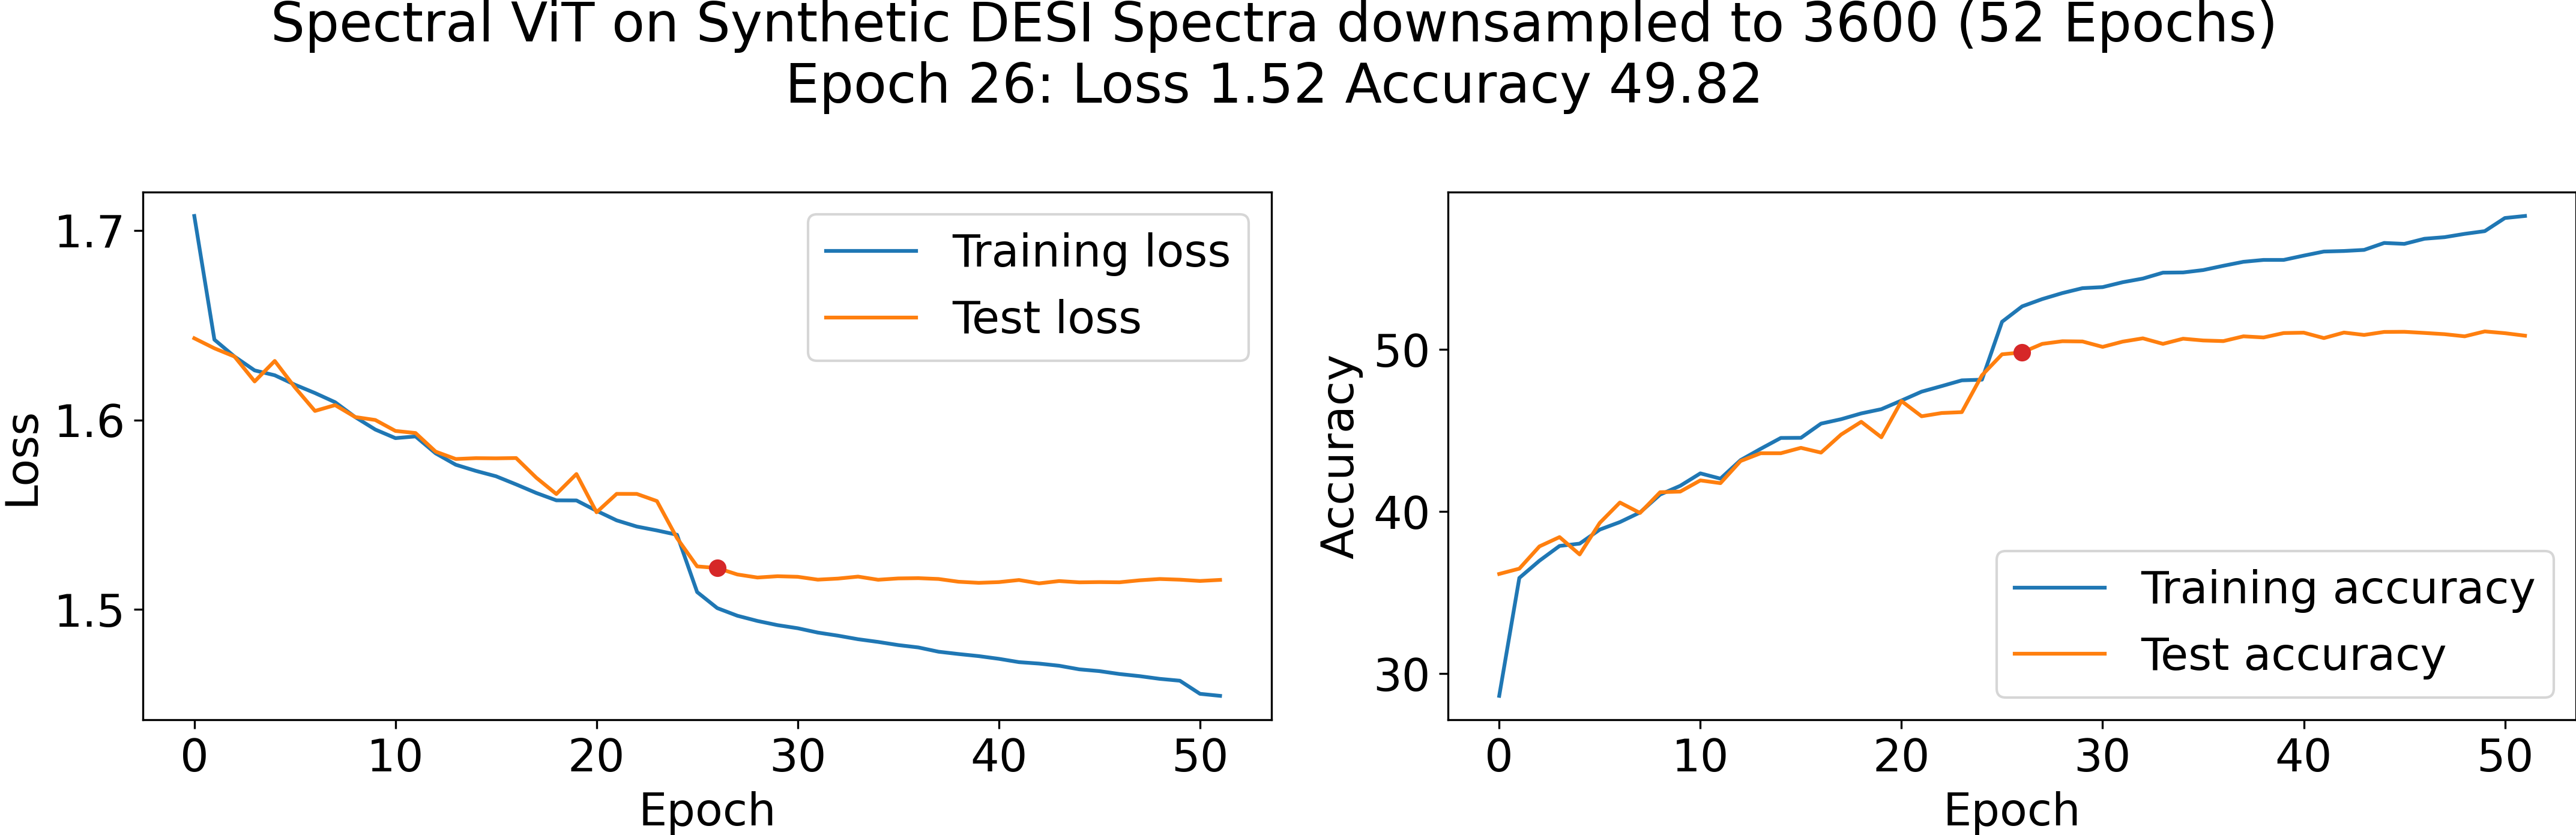
\includegraphics[width=.85\linewidth]{figures/v2_real/vit_model_V2training_new.png}
        \caption[Training of Spectral ViT: V2]{Training of the small architecture on non Redshift-corrected data downsampled to 3600 bins. Over fitting was determined to have occurred by Epoch 26.}
        \label{fig:vit2_training}
    \end{figure}
\end{frame}
\end{comment}




\begin{comment}
%%%%%%%%%%%%%%%%%%%%%%%%%%%%%%%%%%%%%%%%%%%%%%%%%%%%%%%%%%%%%%%%%%%%%%%%
\begin{frame}
    \frametitle{Training}
    \small
    \begin{table}
        \centering
        \caption{HAM10000 Dataset Split}
        \resizebox{\linewidth}{!}{\begin{tabular}{lccc}
	\toprule
    \textbf{Spam} & \textbf{Ni} & \textbf{Swallow} & \textbf{Shrubbery} \\
    \midrule
    A & 1 & 2 & 3 \\
    \midrule
    E & 3 & 4 & 5 \\
    C & 6 & 9 & 3 \\
    \midrule
    M & 4 & 1 & 1 \\
    \bottomrule
\end{tabular}}
    \end{table}
\end{frame}
%%%%%%%%%%%%%%%%%%%%%%%%%%%%%%%%%%%%%%%%%%%%%%%%%%%%%%%%%%%%%%%%%%%%%%%%
\begin{frame}[fragile]
    \frametitle{Verification of Model}
    \begin{block}{Classification}
        Does the predicted class match the true class? 
    \end{block}
    \begin{block}{Segmentation}
    First take the softmax of the outputs (limit from 0 to 1), then compare to true mask
    \begin{exampleblock}{Dice Score}
        \begin{equation}\label{eqn:DiceScore}
            \text{Dice} = \frac{2|X \cap Y|}{|X| + |Y| + \epsilon}
        \end{equation}
        Where $\epsilon$ is a small constant to prevent division by 0. 
    \end{exampleblock}
    
    \end{block}

\end{frame}
\end{comment}